\documentclass[a0]{tumposter}

\usepackage[english]{babel}

\usepackage{blindtext}

\usepackage{xcolor} 
\usepackage{multicol}
\usepackage{amsmath}
\usepackage{graphicx}
\usepackage{tabularx}

\usepackage[utf8]{inputenc}
\usepackage{booktabs}
\usepackage{natbib}
\usepackage{tikz}
\usetikzlibrary{arrows, positioning, 3d, calc, fit}
\usetikzlibrary{spy}
\usetikzlibrary{backgrounds}
\usetikzlibrary{matrix}

\usepackage{pgfplots}
\usepgfplotslibrary{groupplots}
\usepackage{pgfplotstable}
\usepgfplotslibrary{dateplot}

\newcommand{\pre}[1]{
	{\color{focusone}\textbf{#1}}
}
\newcommand{\post}[1]{
	{\color{focustwo}\textbf{#1}}
}


% for printing fontsizes
\usepackage{printlen}
\uselengthunit{mm}

\definecolor{gridcolor}{HTML}{284251}
%\definecolor{focusone}{HTML}{4575b4} % IKB
%\definecolor{focustwo}{HTML}{be3e2b} % IKB

\colorlet{focusone}{tumbluedark}
\colorlet{focustwo}{tumorange}

\colorlet{activationcolor}{focusone} % IKB
\colorlet{contextonecolor}{focustwo!40}
\colorlet{contexttwocolor}{focustwo!60}
\colorlet{contextthreecolor}{focustwo!80}
\colorlet{contextfourcolor}{focustwo}

\tikzstyle{perspective3d}=[z={(0.5cm,-0.5cm)}, x={(1cm,0cm)}, y={(0cm,1cm)}]
\tikzstyle{conn}=[-stealth, semithick, rounded corners]
\tikzstyle{revconn}=[stealth-,semithick,  rounded corners]
\tikzstyle{shared}=[stealth-stealth, rounded corners, very thick]
\tikzstyle{fm}=[inner sep=0]
\tikzstyle{net}=[inner sep=.5em, draw=gridcolor, rounded corners]
\tikzstyle{grid}=[inner sep=0]
\tikzstyle{annotation}=[thin, tumgray, shorten >=1em] % shorten <=1em, 
%\tikzstyle{noteannot}=[draw, rounded corners, align=left, font=\small, draw=tumbluedark, fill=none]
\tikzstyle{noteannot}=[draw, rounded corners, align=left, font=\small, draw=white, fill=tumgraylight, text=tumbluedark]
\def\featurescale{2}

\newcommand{\mygridd}[4]{%
        \def\scale{#1}%
        \def\depth{#2}%
        \def\step{#3}%
        \def\fillcolor{#4}%
        \begin{tikzpicture}[scale=\scale, perspective3d]
            \draw[canvas is xy plane at z=1, fill=\fillcolor,rounded corners=0mm] (0,0) -- (0,1) -- (\depth,1) -- (\depth,0) -- (0,0);
            \draw[canvas is xz plane at y=1, fill=\fillcolor,rounded corners=0mm] (0,0) -- (0,1) -- (\depth,1) -- (\depth,0) -- (0,0);
            \draw[canvas is yz plane at x=0, fill=\fillcolor,rounded corners=0mm] (0,0) -- (0,1) -- (1,1) -- (1,0) -- (0,0);
            \draw[canvas is yz plane at x=0, step=\step, draw=black,rounded corners=0mm] (0,0)  grid (1,1);
        \end{tikzpicture}    
        }%

\newcommand{\concatsone}{
\begin{tikzpicture}
    \node[inner sep=0] at (0,0){\mygridd{\featurescale}{.125}{.25}{activationcolor!70}};
    \node[inner sep=0] at (-.25,0){\mygridd{\featurescale}{.125}{.25}{activationcolor}};
\end{tikzpicture}
}

\newcommand{\concatstwo}{
\begin{tikzpicture}
    \node[inner sep=0] at (0,0){\mygridd{\featurescale}{.125}{.33}{activationcolor!70}};
    \node[inner sep=0] at (-.25	,0){\mygridd{\featurescale}{.125}{.33}{activationcolor}};
\end{tikzpicture}
}

\newcommand{\concatcontext}{
\begin{tikzpicture}
    \node[inner sep=0] at (0,0){\mygridd{\featurescale}{.5}{.25}{activationcolor}};
    \node[inner sep=0] at (-.25,0){\mygridd{\featurescale}{.125}{.25}{contextonecolor}};
    \node[inner sep=0] at (-.5,0){\mygridd{\featurescale}{.125}{.25}{contexttwocolor}};
    \node[inner sep=0] at (-.75,0){\mygridd{\featurescale}{.125}{.25}{contextthreecolor}};
    \node[inner sep=0] at (-1,0){\mygridd{\featurescale}{.125}{.25}{contextfourcolor}};
\end{tikzpicture}
}

\newcommand{\contextfeaturemaps}{
\begin{tikzpicture}[xshift=1]
    \node[inner sep=0] at (-.25,0){\mygridd{\featurescale}{.125}{.25}{contextonecolor}};
	\node[inner sep=0] at (-.5,0){\mygridd{\featurescale}{.125}{.25}{contexttwocolor}};
	\node[inner sep=0] at (-.75,0){\mygridd{\featurescale}{.125}{.25}{contextthreecolor}};
	\node[inner sep=0] at (-1,0){\mygridd{\featurescale}{.125}{.25}{contextfourcolor}};
\end{tikzpicture}
}

\newcommand{\figpspmodule}{
	\begin{tikzpicture}[node distance=.5em, xscale=\featurescale, yscale=-1.5]
	
	\coordinate (legend) at (0,4);
	
	\node[label={below:\scriptsize features}, inner sep=0](input) at (-1.3,1.5) {\mygridd{\featurescale}{.5}{.25}{activationcolor}};
	\node[label={below:\scriptsize context}, inner sep=0](output) at (3.3,1.5) {\contextfeaturemaps};
	
	\coordinate[right=of input] (pool);
	\coordinate[left=of output] (upsample);
	
	\node[inner sep=0](grid1) at (0.2,0){\mygridd{.5}{.5}{.5}{activationcolor!40}};
	\node[inner sep=0](grid2) at (0.2,.8){\mygridd{.75}{.5}{.25}{activationcolor!60}};
	\node[inner sep=0](grid3) at (0.2,1.8){\mygridd{1}{.5}{.25}{activationcolor!80}};
	\node[inner sep=0](grid16) at (0.2,3){\mygridd{1.25}{.5}{.25}{activationcolor}};
	
	\coordinate[below right= 1em and 2em of grid16](convcoord);
	
	%\node(conv1) at (1,0) {conv};
	%\node(conv2) at (1,.8) {conv};
	%\node(conv3) at (1,1.8) {conv};
	%\node(conv16) at (1,3) {conv};
	
	\node[inner sep=0](gridd1) at (1.8,0){\mygridd{.5}{.2}{.5}{contextonecolor}};
	\node[inner sep=0](gridd2) at (1.8,.8){\mygridd{.75}{.2}{.25}{contexttwocolor}};
	\node[inner sep=0](gridd3) at (1.8,1.8){\mygridd{1}{.2}{.25}{contextthreecolor}};
	\node[inner sep=0](gridd16) at (1.8,3){\mygridd{1.25}{.2}{.25}{contextfourcolor}};
	
	\coordinate (center) at ($ (gridd1)!0.5!(grid1) $);
	
	\draw[conn] (input) -- (pool) |- (grid1);
	\draw[conn] (input) -- (pool) |- (grid2);
	\draw[conn] (input) -- (pool) |- (grid3);
	\draw[conn] (input) -- (pool) |- (grid16);
	
	\draw[conn] (grid1) -- (gridd1);
	\draw[conn] (grid2) -- (gridd2);
	\draw[conn] (grid3) -- (gridd3);
	\draw[conn] (grid16) -- (gridd16);
	
	\draw[revconn] (output) -- (upsample) |- (gridd1);
	\draw[revconn] (output) -- (upsample) |- (gridd2);
	\draw[revconn] (output) -- (upsample) |- (gridd3);
	\draw[revconn] (output) -- (upsample) |- (gridd16);
	
	\node[anchor=mid](legpool) at (legend -| pool) {\scriptsize pooling};
	\node[anchor=mid](legupsampl) at (legend -| upsample) {\scriptsize upsampl.};
	\node[anchor=mid](legconv) at (legend -| center) {\scriptsize conv.};
	
	%\node[draw, rounded corners, label={[align=center]below:Pyramid Spatial Pooling (PSP) \\ Module}, fit=(input)(grid1)(gridd16)(output)(legpool)(legupsampl)(legconv)]{};

	\end{tikzpicture}
}

\newcommand{\figFusionNetwork}{
\def\imagewidth{4cm}
	
\begin{tikzpicture}[node distance=0.5em, yscale=4.5]

    \def\labelimage{images/networkoutputbuildings}
    
    %% Sentinel-1
    \node[inner sep=0, label={[anchor=south, rotate=90,label distance=0em]left:\scriptsize pre}] at (0,3.03) (s1pre) {
\includegraphics[width=\imagewidth]{images/s1pre}};
    \node[inner sep=0, label={[anchor=south, rotate=90,label distance=0em]left:\scriptsize post}] at (0,3.97) (s1post) {
\includegraphics[width=\imagewidth]{images/s1post}};
    %\node[anchor=east, rotate=0] at (-3,3.5) {\small Sentinel-1};

    \coordinate (center) at ($ (s1pre.east)!0.5!(s1post.east) $);
    \node[right=of center, inner sep=0, label={[anchor=center, label distance=1em]below right:\scriptsize 192px}] (minusone) {\concatsone};

    \node[net,right=of minusone, fill=white] (resnet) {\small ResNet};
    \node[right=of resnet, inner sep=0, label={[anchor=center, label distance=.4em]below:\scriptsize 96px}] (h0) {\mygridd{\featurescale}{.5}{.25}{activationcolor}};
    \node[net, right=of h0, align=left, fill=white] (pspmodule) {\small PSP Module};
    \node[right=of pspmodule, inner sep=0, label={[anchor=center, label distance=.4em]below:\scriptsize 96px}] (aggrout) {\concatcontext};
    \node[right=of aggrout, inner sep=0] (s1label) {\includegraphics[width=\imagewidth]{\labelimage}};

    \draw[conn] (s1pre.east)++(0,-.1em) -| (minusone);
    \draw[conn] (s1post.east)++(0,.1em) -| (minusone);
    \draw[conn] (minusone) -- (resnet);
    \draw[conn] (resnet) -- (h0);
    \draw[conn] (h0) -- (pspmodule);
    \draw[conn] (pspmodule) -- (aggrout);
    \draw[conn] (aggrout) -- (s1label);
    \draw[conn] (h0) |- ++(1em,.5em) -| (aggrout);

	
    %% Sentinel-2
    \node[inner sep=0, label={[label distance=0em, anchor=south, rotate=90]left:\scriptsize pre}] at (0,1.03) (s2pre) {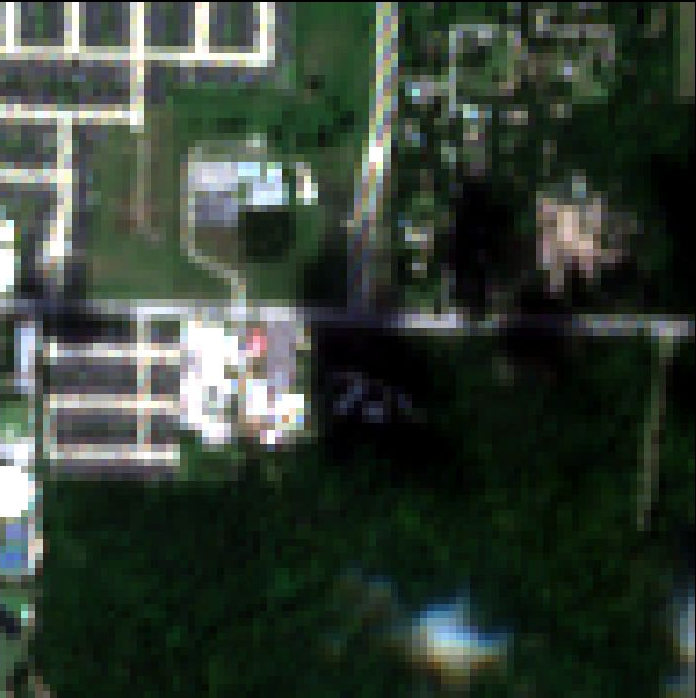
\includegraphics[width=\imagewidth]{images/s2pre}};
    \node[inner sep=0, label={[anchor=south, rotate=90,label distance=0em]left:\scriptsize post}] at (0,1.97) (s2post) {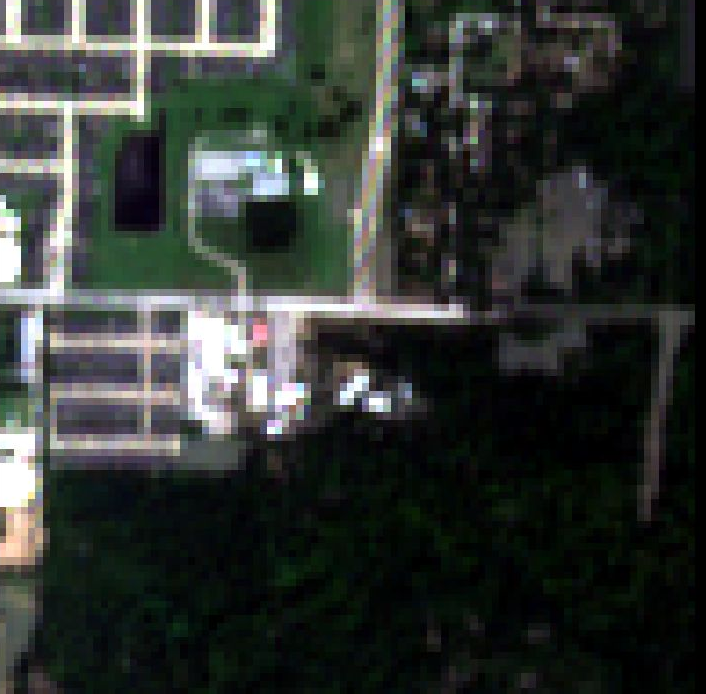
\includegraphics[width=\imagewidth]{images/s2post}};
    %\node[anchor=east, rotate=0] at (-3,1.5) {\small Sentinel-2};

    \coordinate (center) at ($ (s2pre.east)!0.5!(s2post.east) $);
    \node[right=of center, inner sep=0, label={[anchor=center,label distance=1em]below right:\scriptsize 96px}] (minus) {\concatstwo};
    \node[net,right=of minus, fill=white] (resnet) {\small ResNet};
    \node[right=of resnet, inner sep=0, label={[anchor=center, label distance=.4em]below:\scriptsize 96px}] (h0) {\mygridd{\featurescale}{.5}{.25}{activationcolor}};
    \node[net, right=of h0, align=left, fill=white] (pspmodule) {\small PSP Module};
    \node[right=of pspmodule, inner sep=0, label={[anchor=center, label distance=.4em]below:\scriptsize 96px}] (aggrout) {\concatcontext};
    \node[right=of aggrout, inner sep=0] (s2label) {\includegraphics[width=\imagewidth]{\labelimage}};

    \draw[conn] (s2pre.east)++(0,-.1em) -| (minus);
    \draw[conn] (s2post.east)++(0,.1em) -| (minus);
    \draw[conn] (minus) -- (resnet);
    \draw[conn] (resnet) -- (h0);
    \draw[conn] (h0) -- (pspmodule);
    \draw[conn] (pspmodule) -- (aggrout);
    \draw[conn] (aggrout) -- (s2label);
    \draw[conn] (h0) |- ++(1em,.5em) -| (aggrout);

	
    %% VHR
    \node[inner sep=0, label={[anchor=south, rotate=90,label distance=0em]left:\scriptsize post}] (input) at (0,-.15) {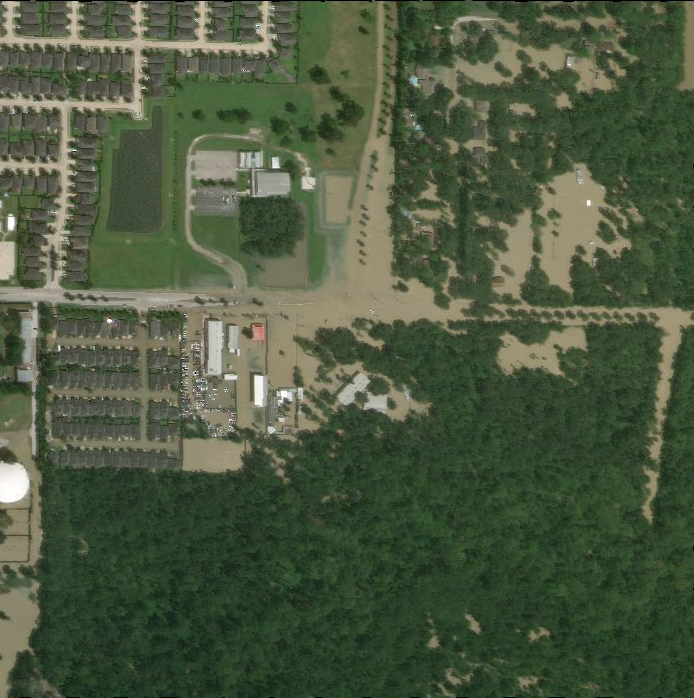
\includegraphics[width=\imagewidth]{images/networkinput}};
    \node[right=of input, inner sep=0, label={[anchor=center, label distance=.4em]below:\scriptsize 1560px}] (hm1) {\mygridd{\featurescale}{.125}{.125}{activationcolor}};
    \node[net,right=of hm1, fill=white] (resnet) {\small ResNet};
    \node[right=of resnet, inner sep=0, label={[anchor=center, label distance=.4em]below:\scriptsize 96px}] (h0) {\mygridd{\featurescale}{.5}{.25}{activationcolor}};
    \node[net,right=of h0, align=left, fill=white] (pspnet) {\small PSP Module};
    \node[right=of pspnet, inner sep=0, label={[anchor=center, label distance=.4em]below:\scriptsize 96px}] (aggrout) {\concatcontext};
    \node[right=of aggrout, align=left, inner sep=0] (pspout) {\includegraphics[width=\imagewidth]{\labelimage}};
    
    \draw[conn] (input.east) -- (hm1);
    \draw[conn] (hm1) -- (resnet);
    \draw[conn] (resnet) -- (h0);
    \draw[conn] (h0) -- (pspnet);
    \draw[conn] (pspnet) -- (aggrout);
    \draw[conn] (aggrout) -- (pspout);
    \draw[conn] (h0) |- ++(1em,.4em) -| (aggrout);

%    \node[anchor=east, rotate=0] at (-3,-.15) {\small very high res.};

    \node[right=2em of s2label](out){\includegraphics[width=\imagewidth]{\labelimage}};
    
    \draw[conn] (s2label) -- (out);
    \draw[conn] (s1label) -| ($ (s1label.east)!0.5!(out.west) $) |- (out.west);
    \draw[conn] (pspout) -| ($ (pspout.east)!0.5!(out.west) $) |- (out.west);
    
    \begin{scope}[on background layer]
    \node[fill=focusone!10, rounded corners, fit=(s1pre)(s1post)(s1label), label={[xshift=-1.5em, anchor=center, rotate=90]left:\small Sentinel 1}, inner sep=.2em]{};
    \node[fill=focusone!10, rounded corners, fit=(s2pre)(s2post)(s2label), label={[xshift=-1.5em, anchor=center, rotate=90]left:\small Sentinel 2}, inner sep=.2em]{};
    \node[fill=focusone!10, rounded corners, fit=(input)(pspout), label={[xshift=-1.5em, anchor=center, rotate=90]left:\small very high res.}, inner ysep=.5em, inner xsep=.2em]{};
   	\end{scope}
    
    %% Annotations
    
    \node[noteannot, below=3cm of pspnet, xshift=1em, draw=none](annotpspnettext){\textbf{pyramid-sampling} \\ \textbf{pooling (PSP)} \\ module aggregates \\ contextual information \\ with multiple pooling \\ convolution, unpooling \\ steps};
    \node[xshift=9em, yshift=0em, draw=none] at (annotpspnettext)(annotpspnetfigure){\figpspmodule};
    \node[below=0em of annotpspnettext, xshift=5cm, text width=20cm, noteannot, draw=none](citepspnet){\verytiny\baselineskip=5pt Zhao, H., Shi, J., Qi, X., Wang, X., \& Jia, J. (2017). \textbf{Pyramid scene parsing network.} IEEE Conf. on CVPR.\par};
    
    \begin{scope}[on background layer]
    \node[noteannot, fit=(annotpspnetfigure)(annotpspnettext)(citepspnet), rounded corners](annotpspnet){};
    
    \draw[annotation] (annotpspnet) -- (pspnet);
    
    \node[below=3cm of resnet, xshift=-3em, noteannot, text width=10cm](annotresnet){\textbf{residual network} \\ serves as encoder to \\ extract features \\ and harmonize \\ resolutions \\ \vspace{1em}
    \verytiny\baselineskip=5pt Szegedy, C., Ioffe, S., Vanhoucke, V., \& Alemi, A. A. (2017). \textbf{Inception-v4, inception-resnet and the impact of residual connections on learning}. In AAAI (Vol. 4, p. 12).\par};
    \draw[annotation] (annotresnet) -- (resnet);
    
    \node[noteannot, yshift=1em, right=2em of s1label](annotstreams){%
    	\textbf{late fusion} \\
    	of independent \\ 
    	streams for each \\ 
    	modality
    };
	\draw[annotation] (annotstreams) -- (s1label);
    \draw[annotation] (annotstreams) -- (s2label);
    %\draw[annotation] (annotstreams) -- (pspout); 
    
    \node[noteannot, xshift=2em, below=2em of out](annotout){%
    	\textbf{prediction} of \\
    	buildings \\ 
    	or flooded build.
    };
	\draw[annotation] (annotout) -- (out); 
	
	\node[noteannot,above=2.5em of minusone, xshift=9em](annotprepost){%
		\textbf{early fusion}
		of pre-event
		and post-
		event images
	};
	\draw[annotation] (annotprepost.south)++(-6em,0) -- (minusone); 
%	\draw[annotation] (annotprepost.south)++(-6em,0) -- (minus); 
	
	\end{scope}
    
    
\end{tikzpicture}
}
\def\imagewidth{5cm}

\newcommand{\figqualitativehouston}{
\begin{tikzpicture}[node distance=.5em]

\node[inner sep=0, label=Sentinel-2 input] (a) {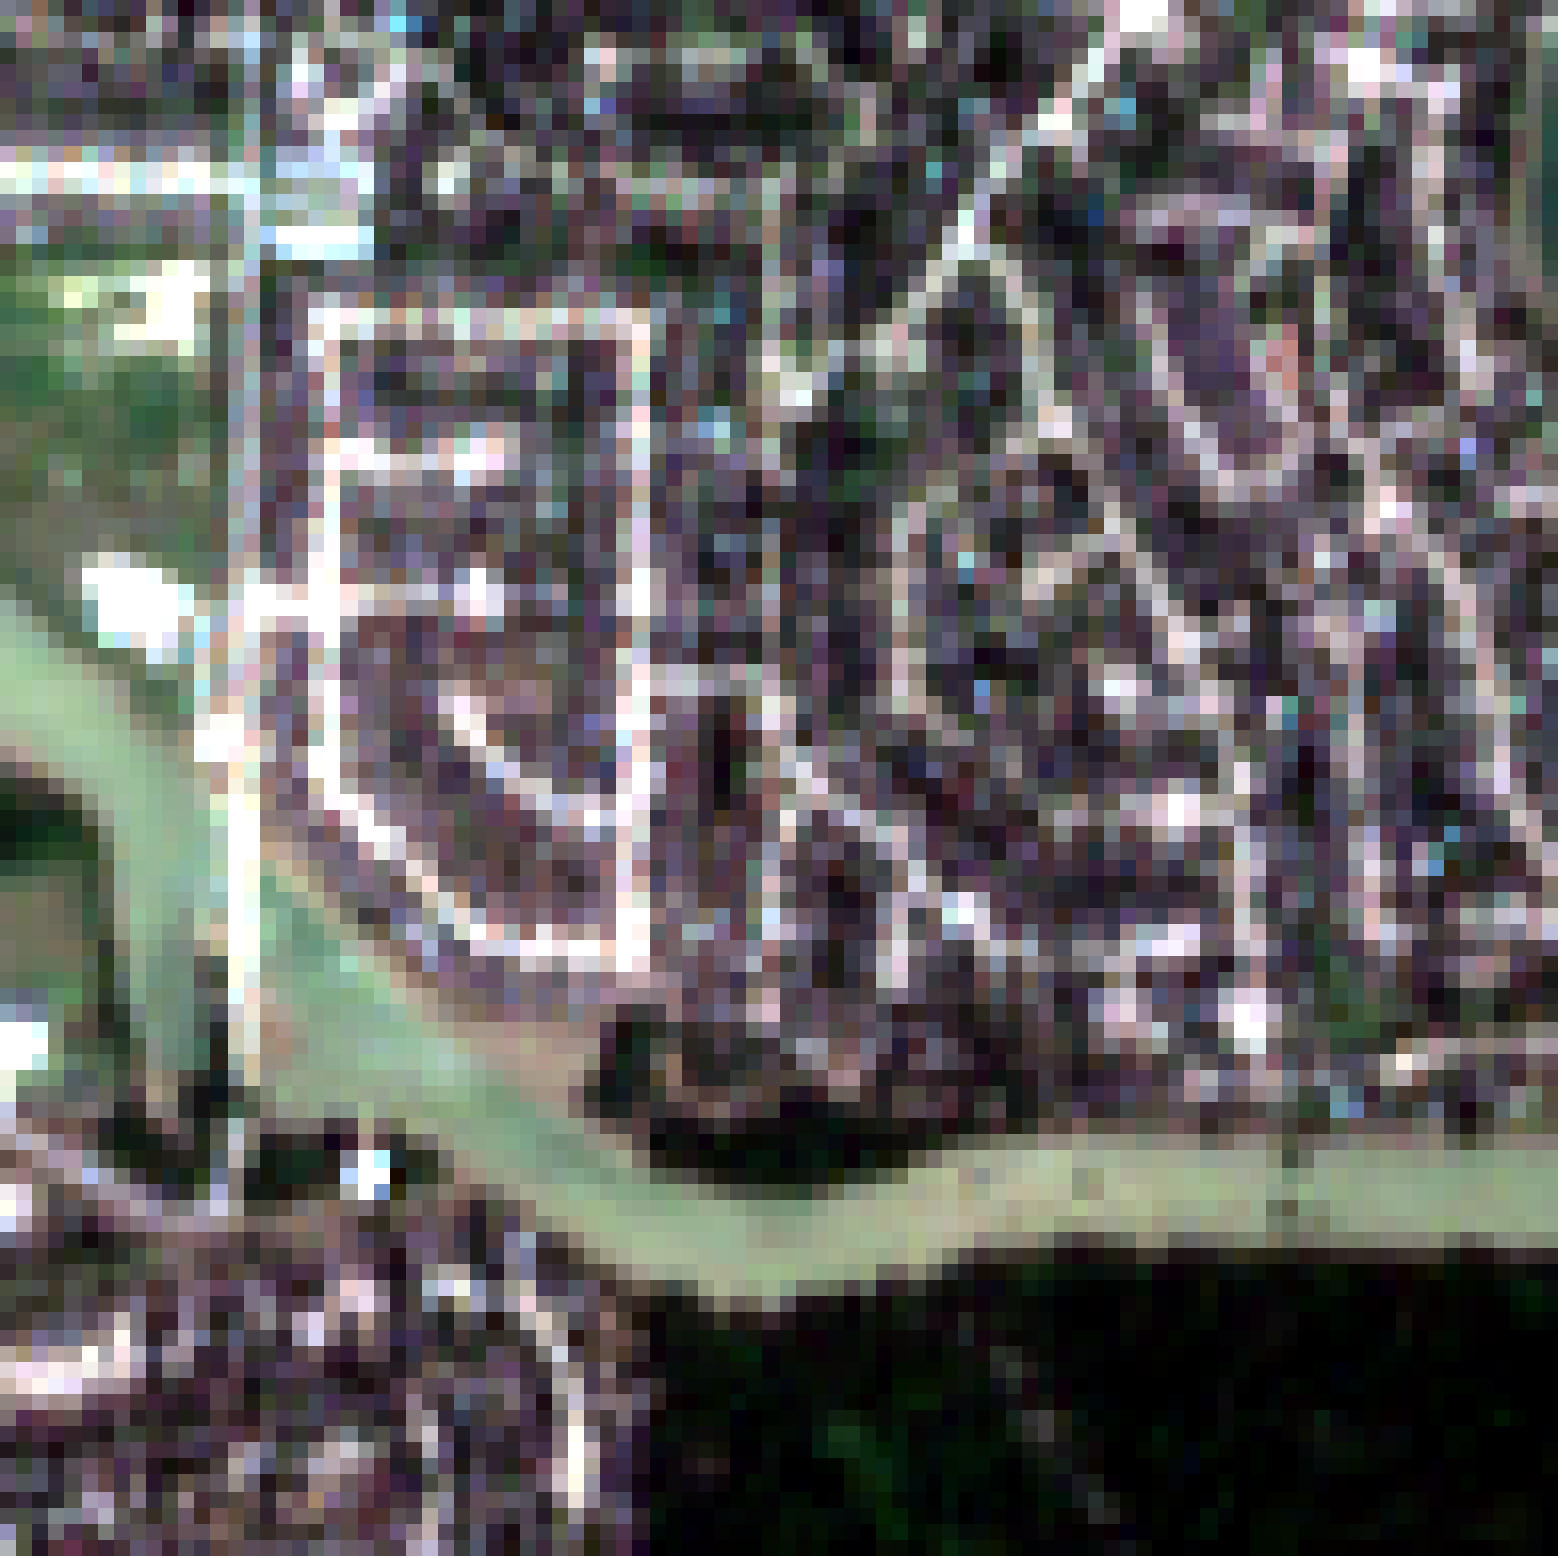
\includegraphics[width=\imagewidth]{images/aaaiqualitative/input_sen.png}};
\node[inner sep=0, right=of a, label=target (10m)] (b) {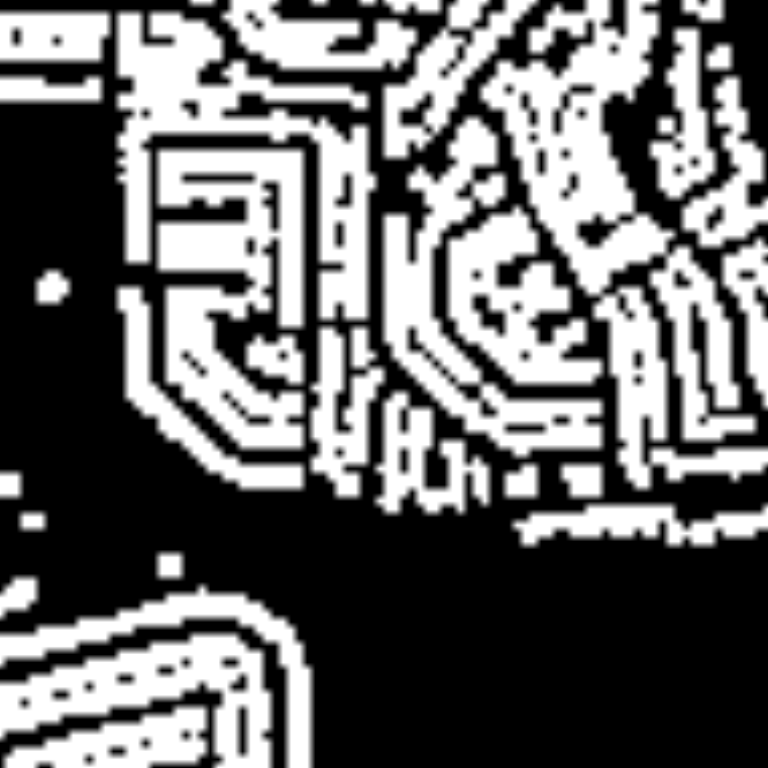
\includegraphics[width=\imagewidth]{images/aaaiqualitative/0_target_class_02_sen.png}};
\node[inner sep=0, right=of b,label=prediction] (c) {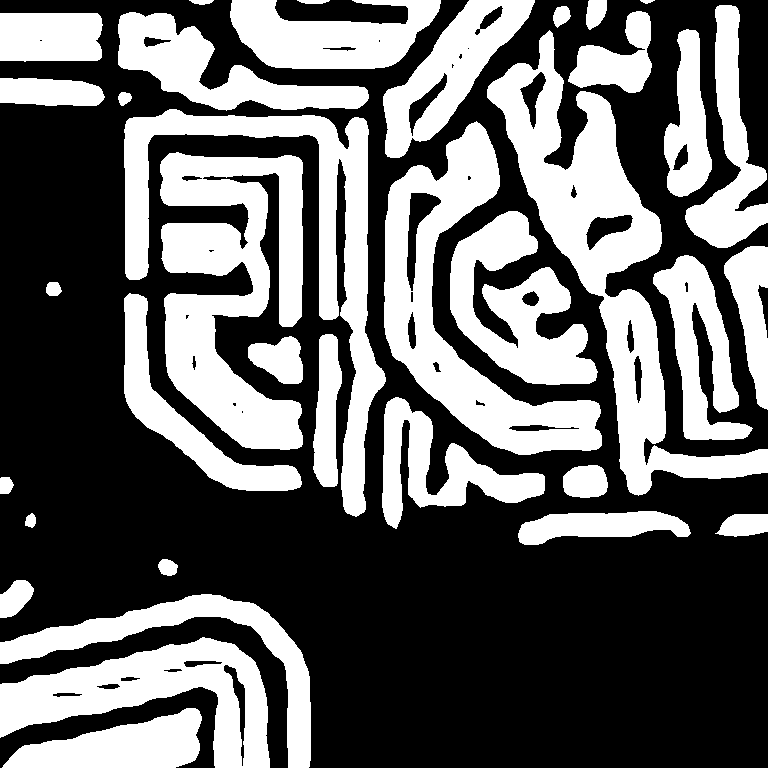
\includegraphics[width=\imagewidth]{images/aaaiqualitative/0_prediction_class_02_sen.png}};


\node[inner sep=0, right= of c, label=VHR input] (a2) {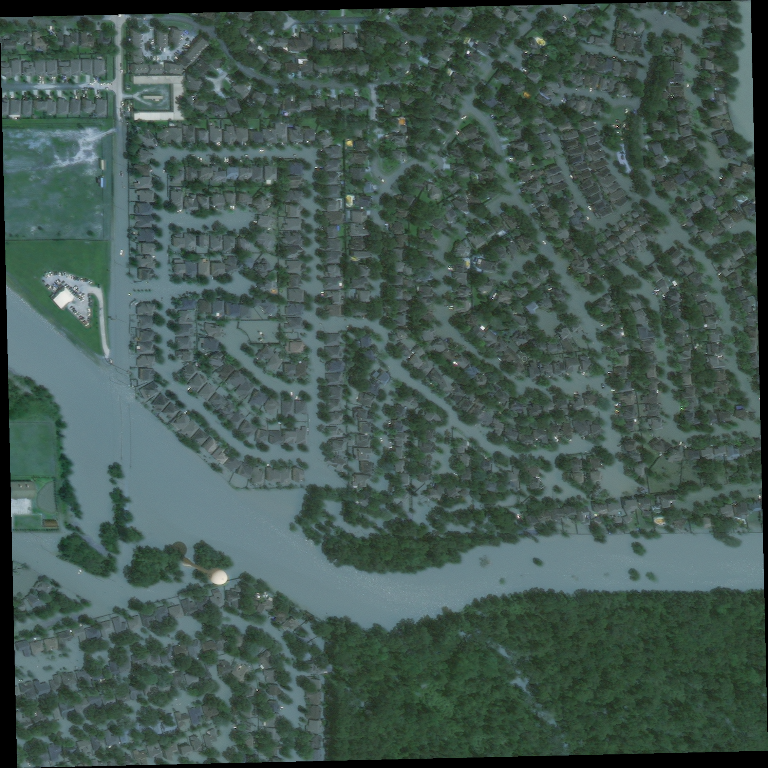
\includegraphics[width=\imagewidth]{images/aaaiqualitative/0_building_input.png}};
\node[inner sep=0, right=of a2, label=target (2m)] (b2) {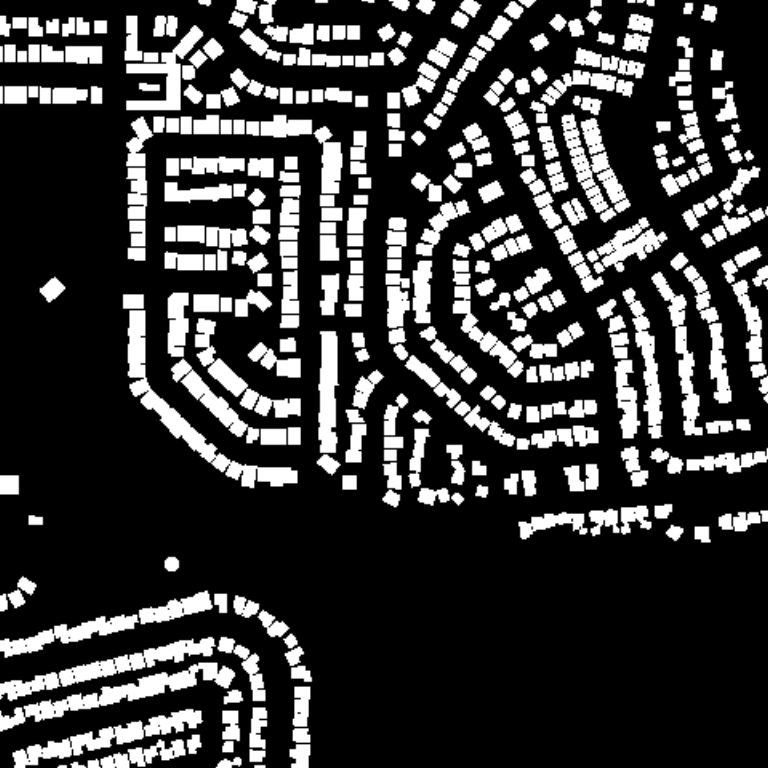
\includegraphics[width=\imagewidth]{images/aaaiqualitative/0_building_target_02.png}};
\node[inner sep=0, right=of b2,label=prediction] (c2) {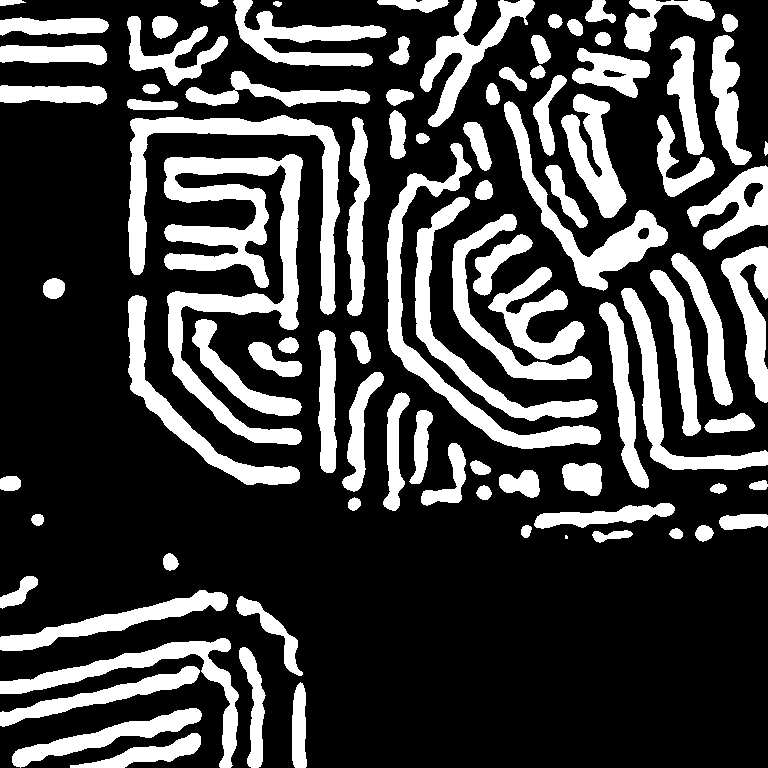
\includegraphics[width=\imagewidth]{images/aaaiqualitative/0_building_prediction.png}};

\coordinate (break) at ($(c)!0.5!(a2)$);
\draw[thick] ($ (break) - (0,1.6cm) $) -- ($ (break) + (0,1.6cm) $) node[at end, above=3em]{};

\end{tikzpicture}
}

\newcommand{\figqualitativefusionhouston}{
\begin{tikzpicture}[node distance=.5em]
\node[inner sep=0, label=VHR input] (a) {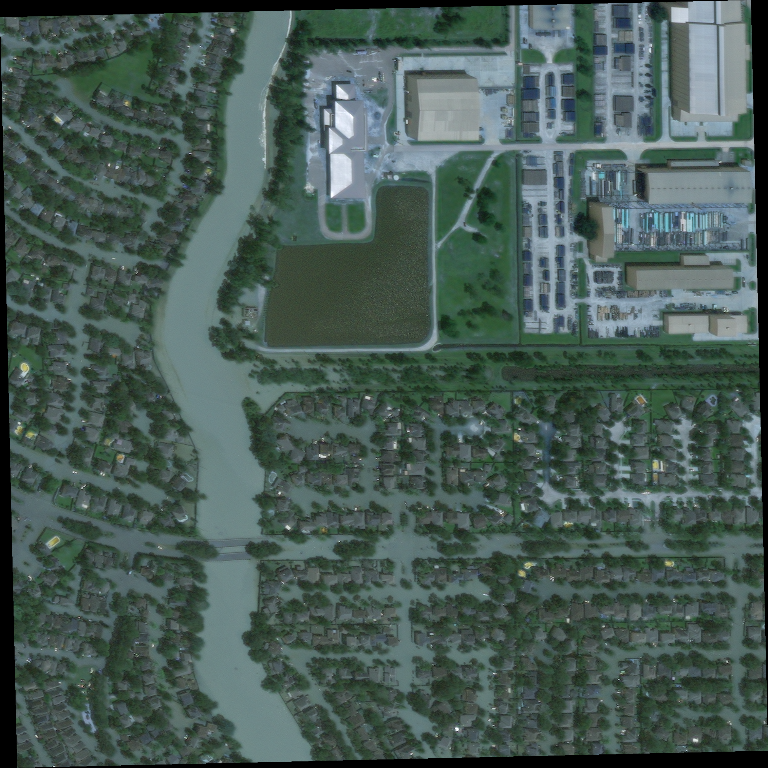
\includegraphics[width=\imagewidth]{images/aaaiqualitative/118_damage_input.png}};
\node[inner sep=0, right=of a, label=target] (b) {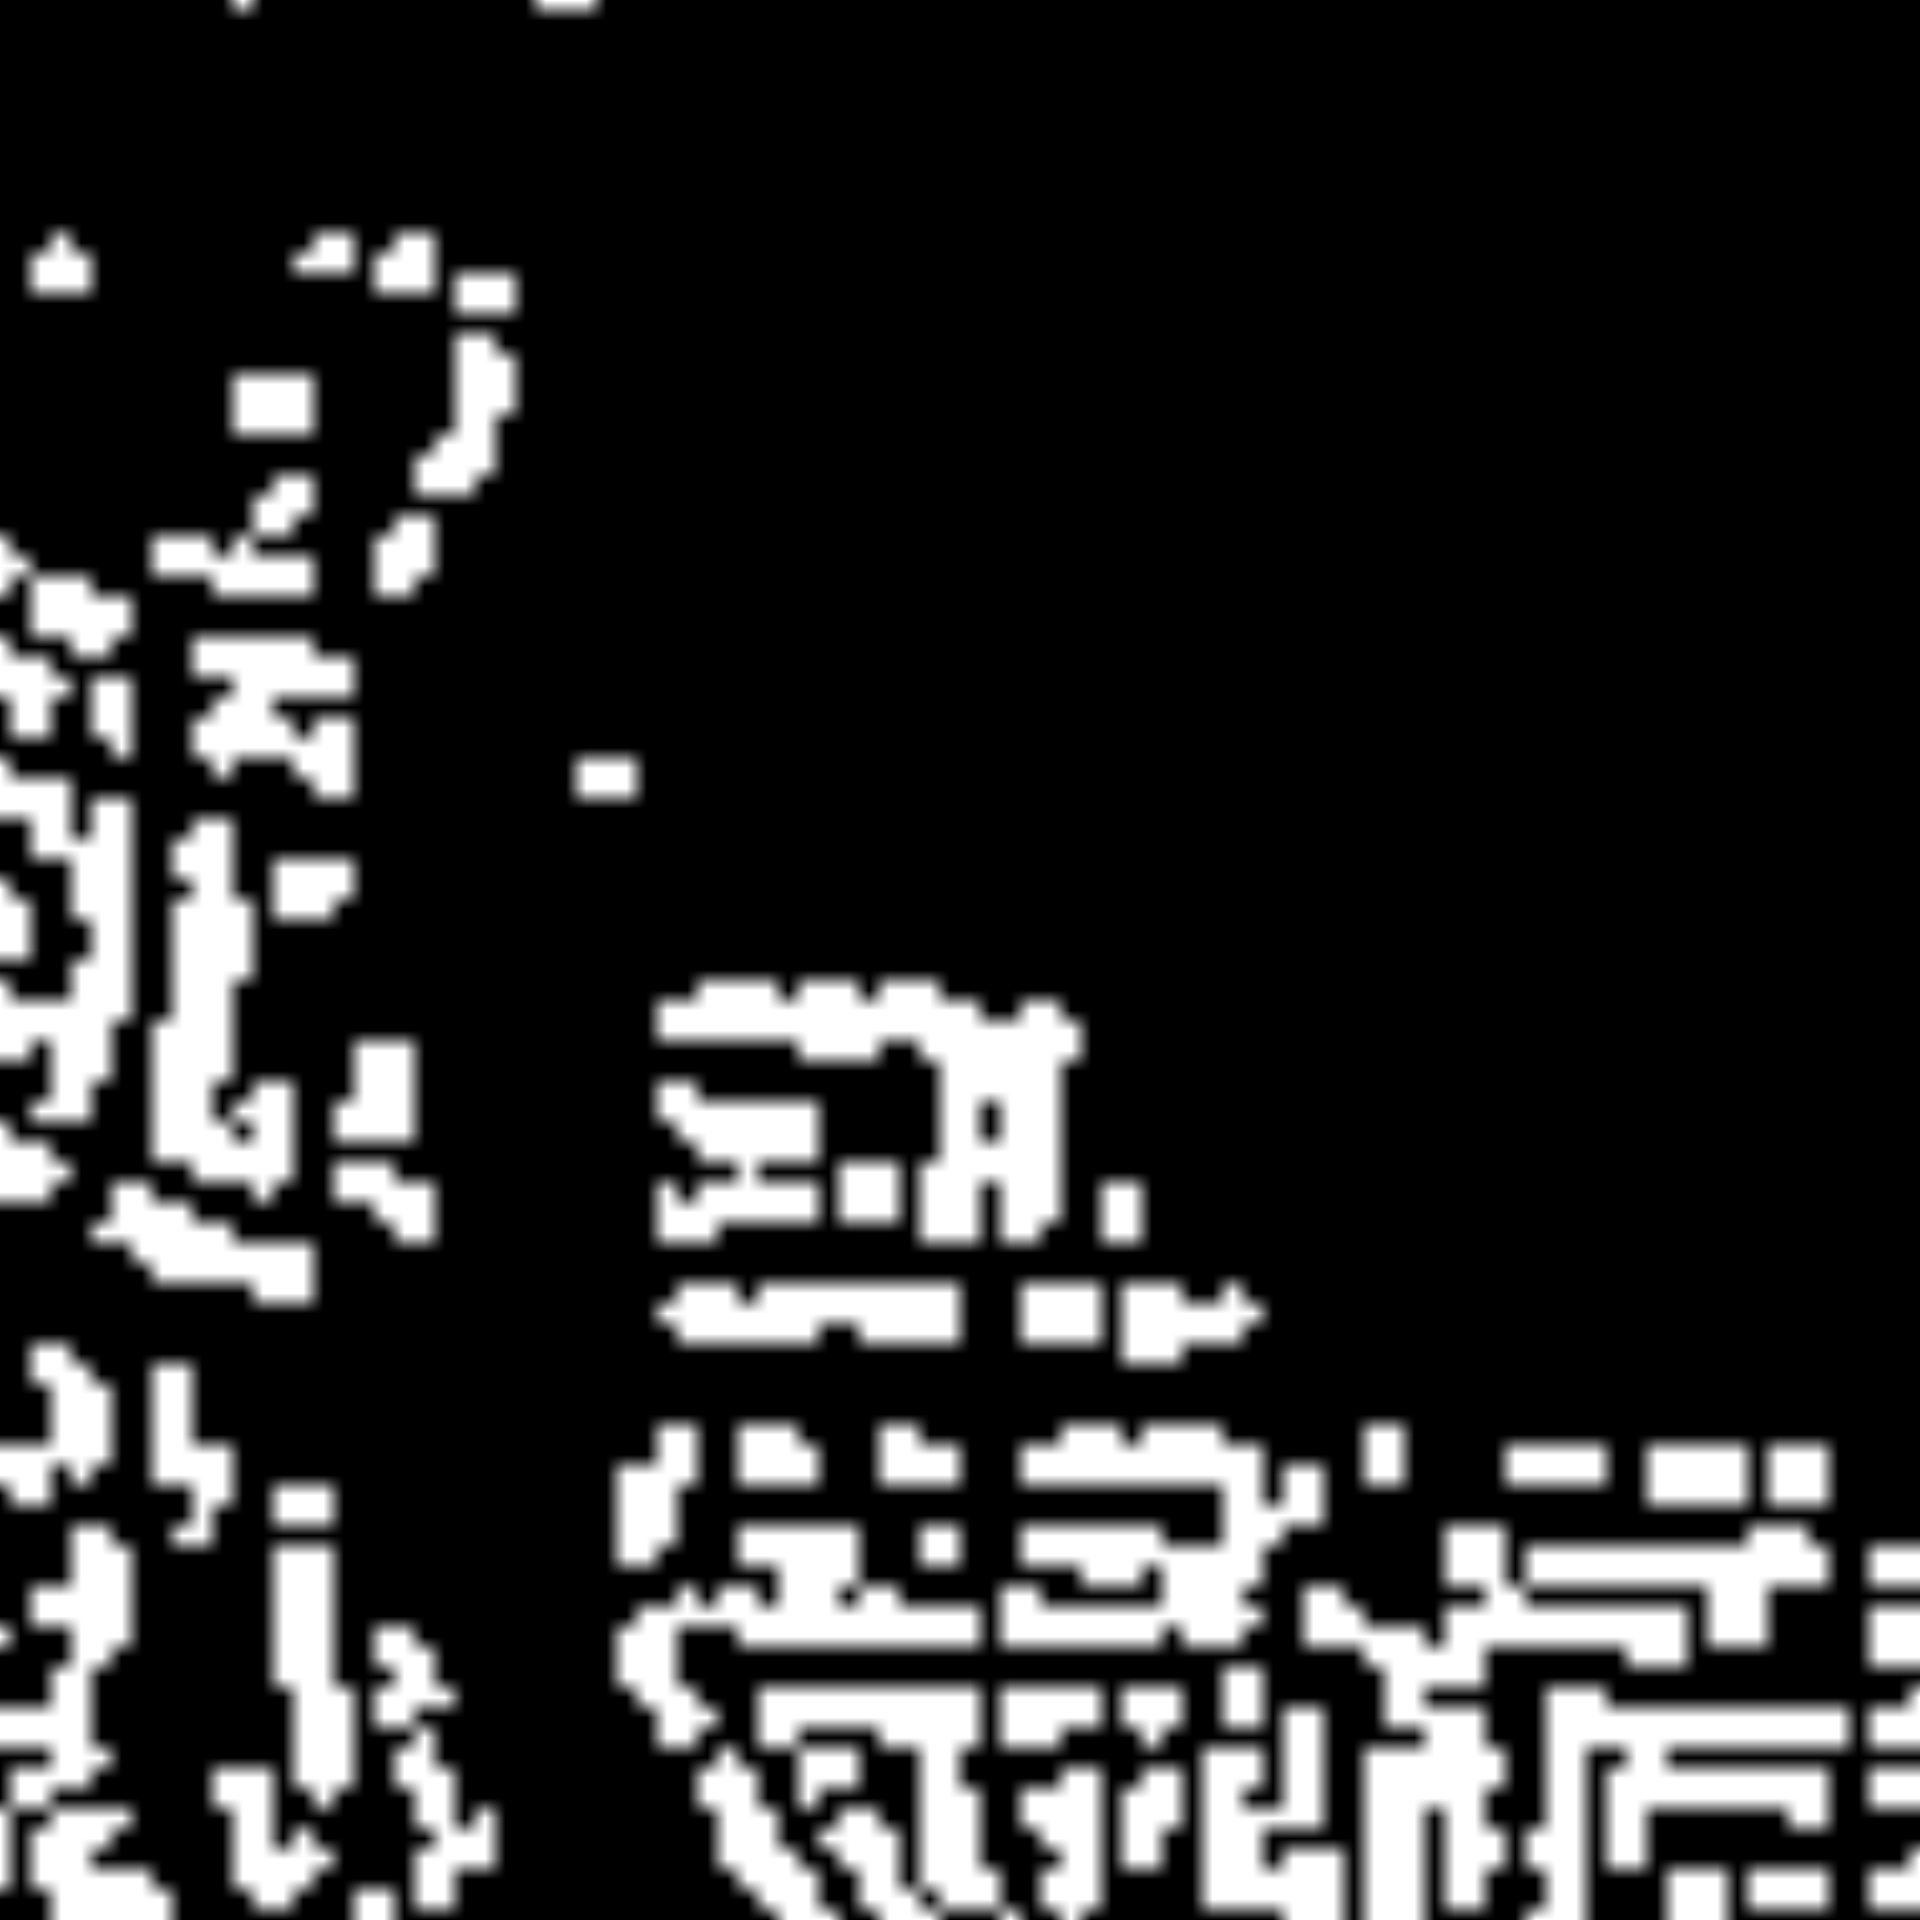
\includegraphics[width=\imagewidth]{images/aaaiqualitative/118_damage_target.png}};
\node[inner sep=0, right=of b,label=fusion prediction] (c) {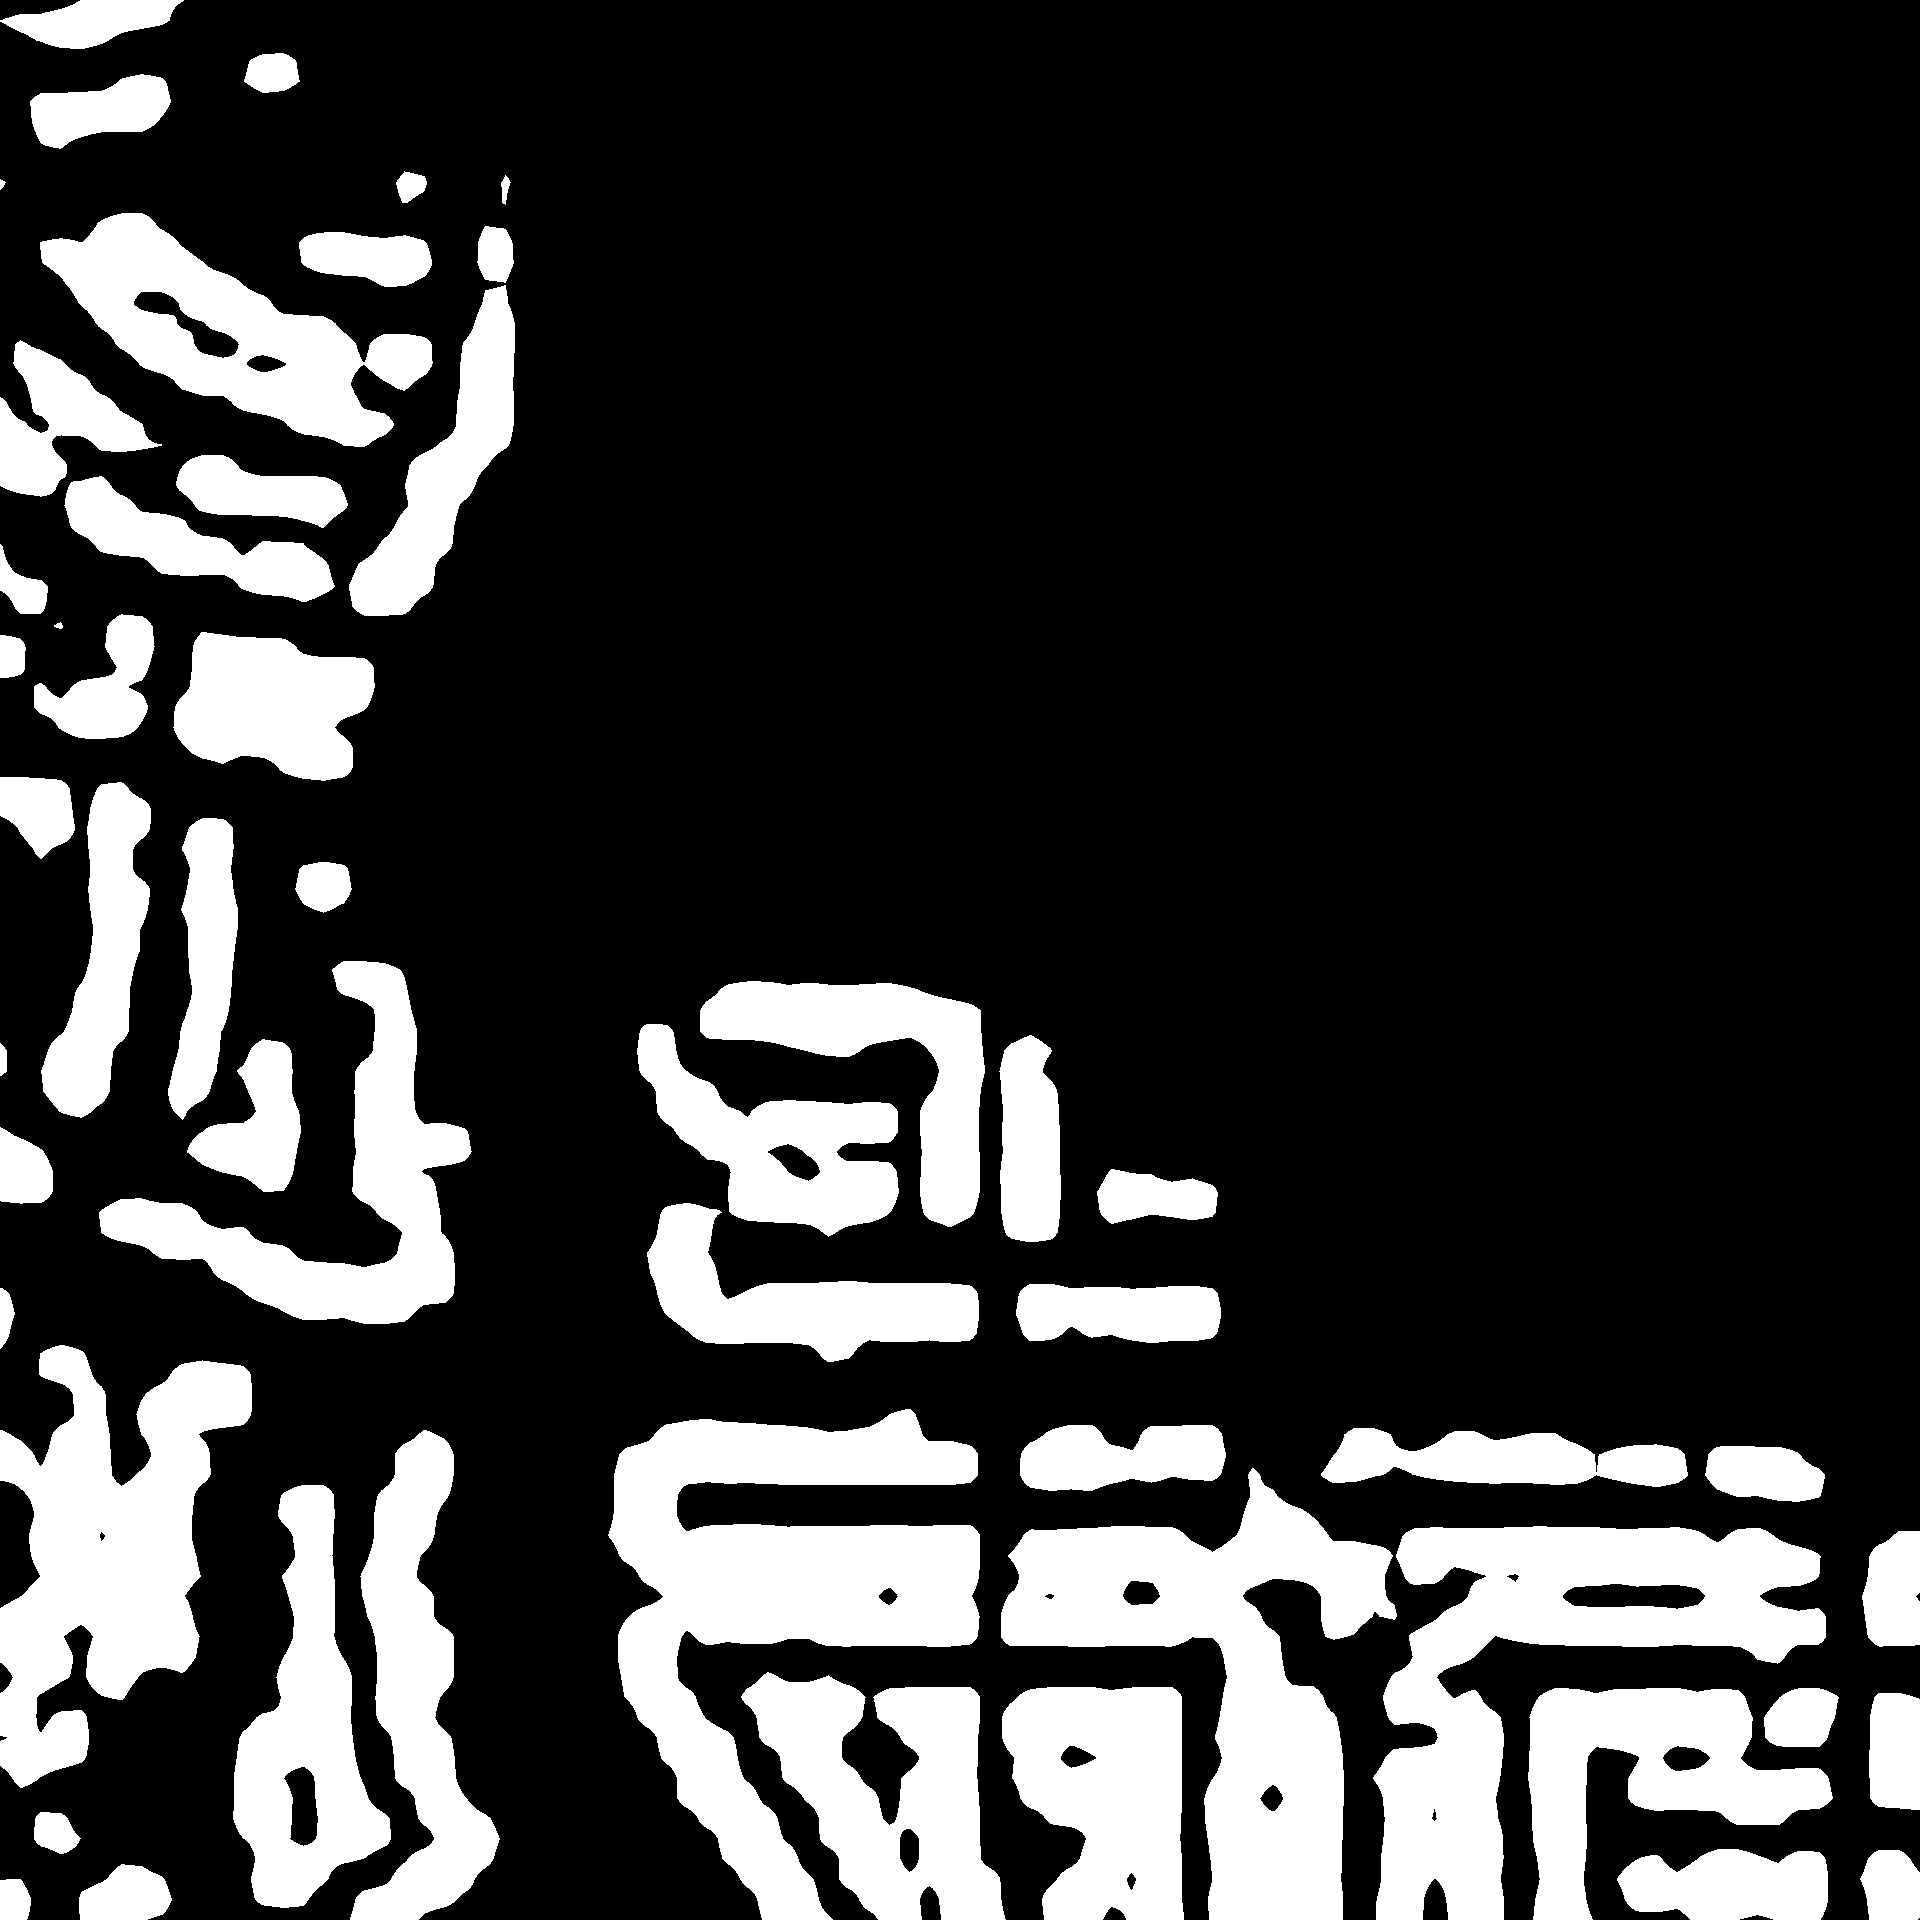
\includegraphics[width=\imagewidth]{images/aaaiqualitative/118_damage_preds_all.png}};


\node[inner sep=0, right=of c, label=VHR only prediction] (d) {
\includegraphics[width=\imagewidth]{images/aaaiqualitative/118_damage_preds_vhr.png}};
\node[inner sep=0, right=of d,label=overlay] (e) {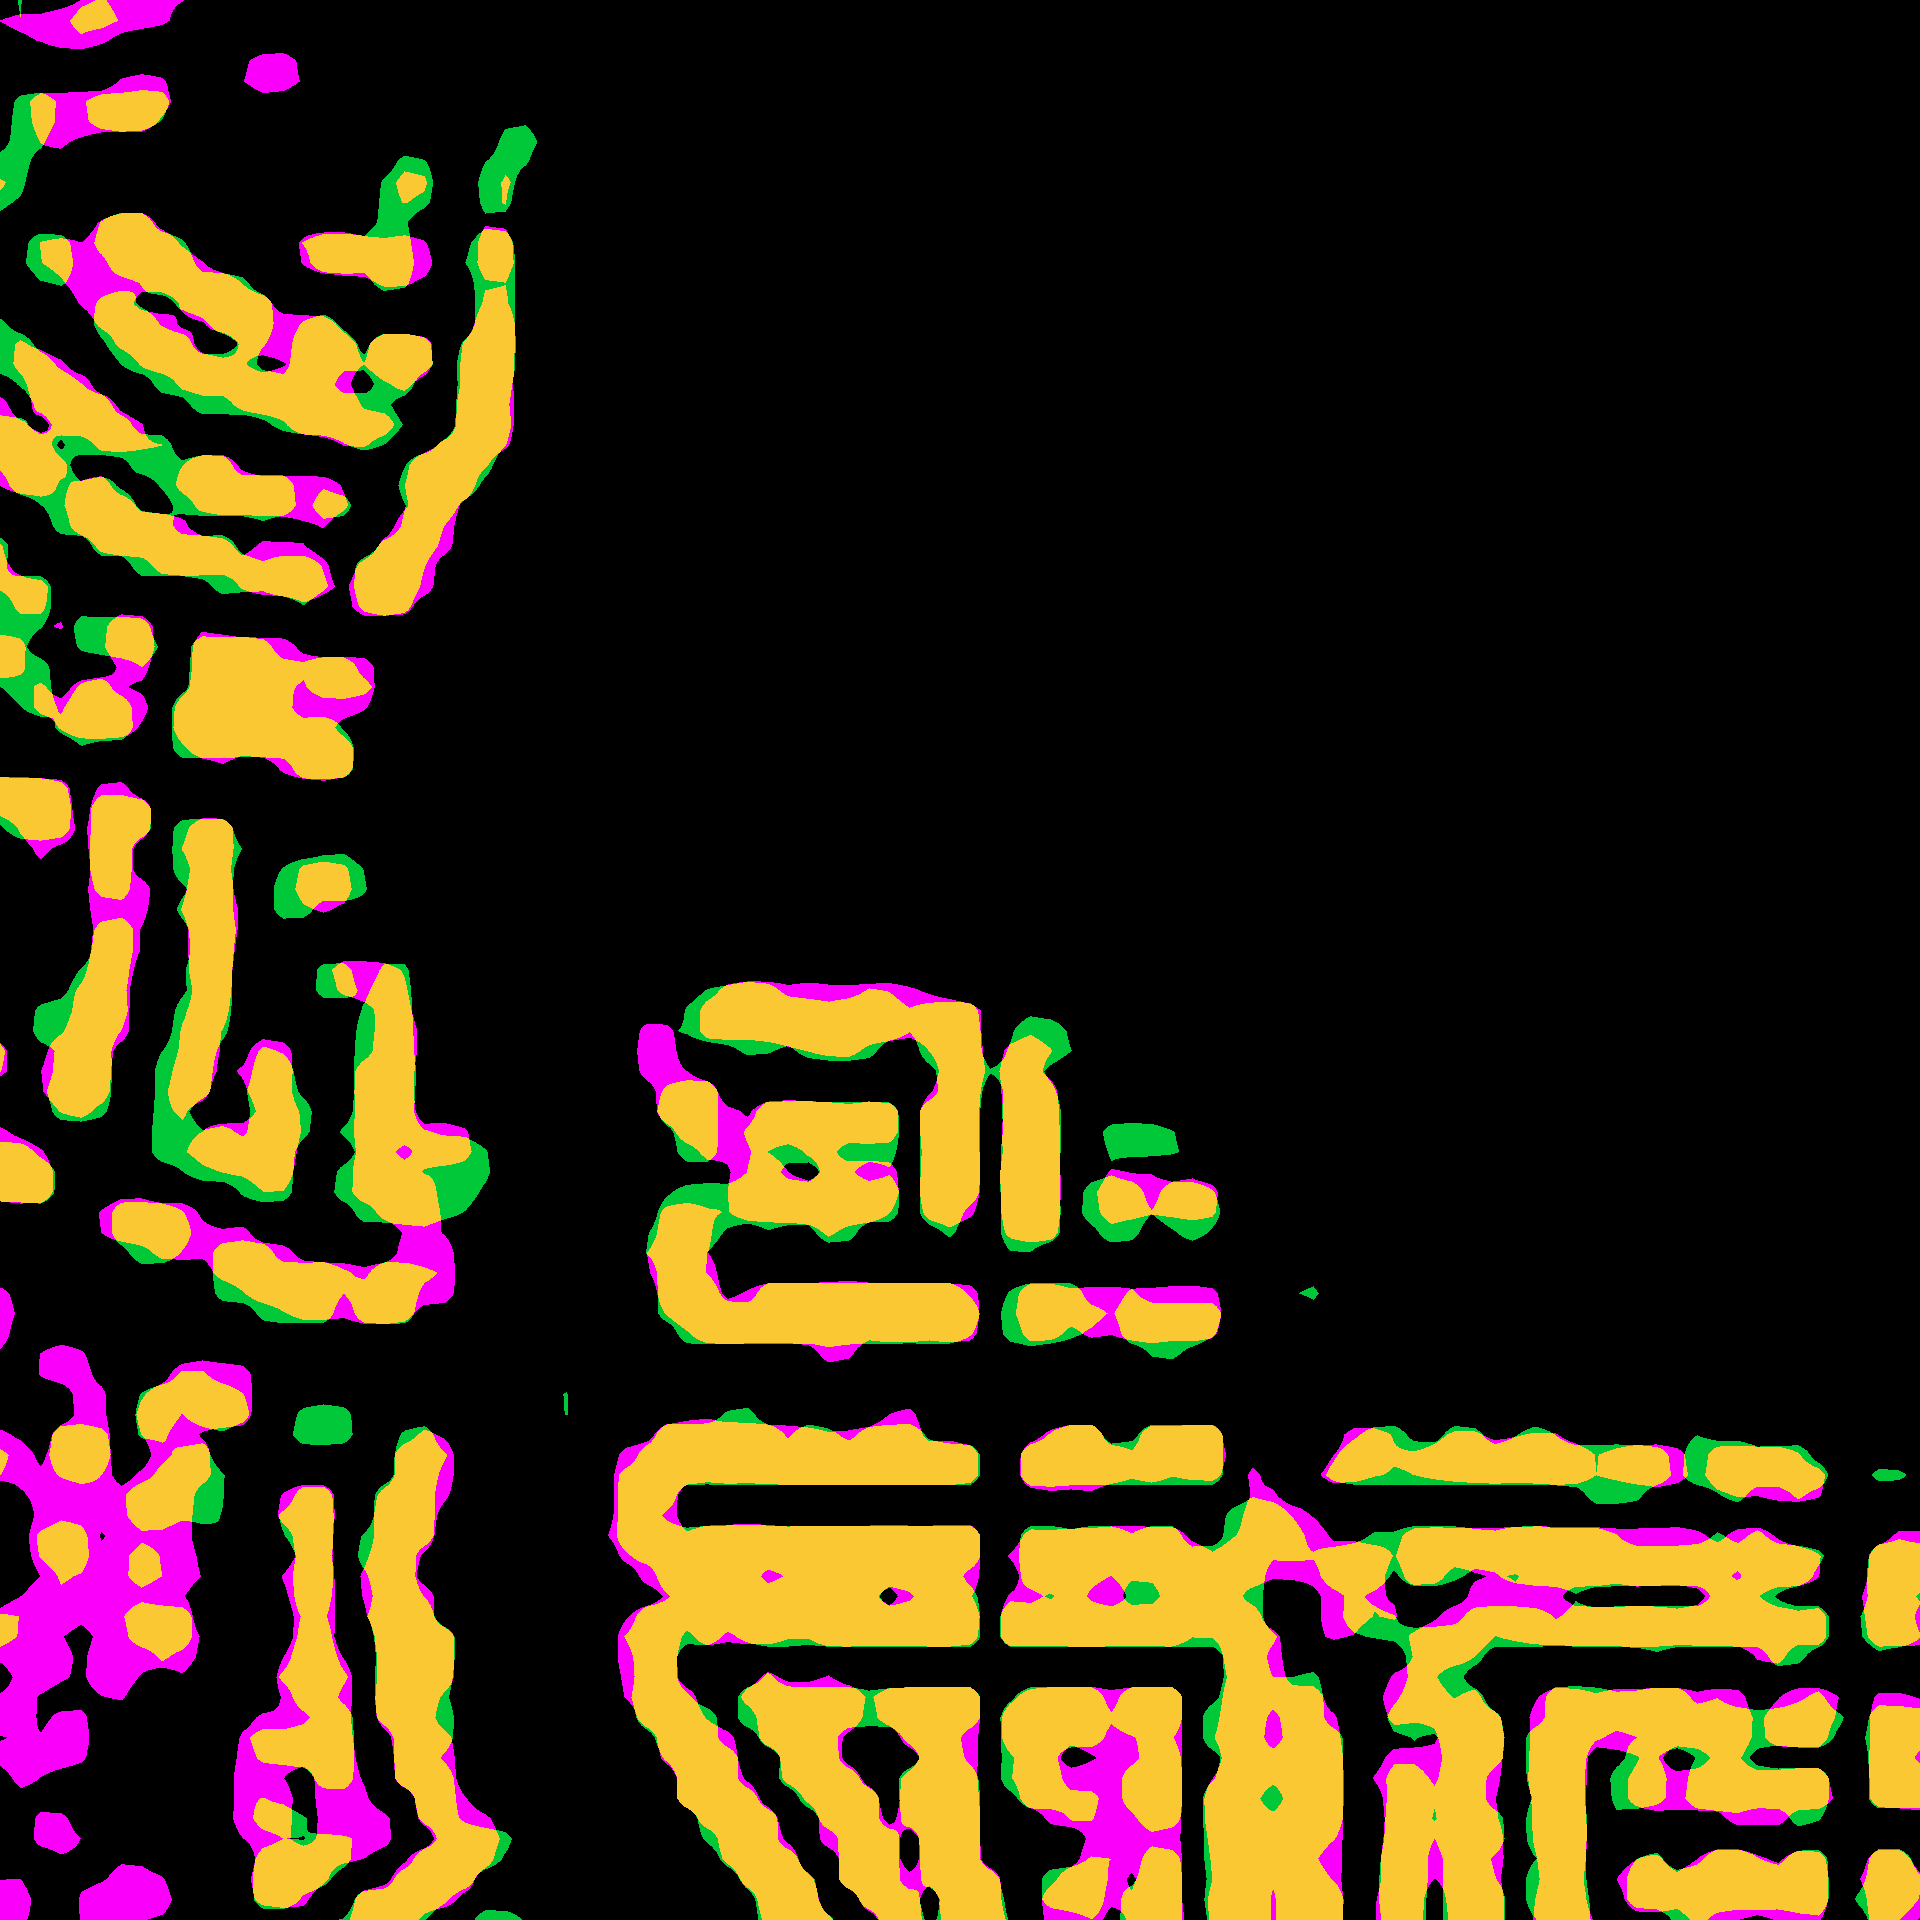
\includegraphics[width=\imagewidth]{images/aaaiqualitative/118_damage_preds_vhr_diff.png}};
\end{tikzpicture}
}

\newcommand{\theteam}{
\begin{tikzpicture}
[node distance=.5em, label distance=.3em]
\node[label={\veryverytiny Marc Ru\ss wurm}](marc){\includegraphics[height=1.52em]{images/team/marc2.jpg}};
\node[right=of marc, label={\veryverytiny Ramona Pelich}](ramona){\includegraphics[width=2.5em]{images/team/rpelich2018.jpg}};
\node[right=of ramona, label={\veryverytiny Ben Bischke}](ben){\includegraphics[width=2.5em]{images/team/portrait_ben.jpg}};
\node[right=of ben, label={\veryverytiny Jakub Fil}](jakub){\includegraphics[width=2.5em]{images/team/headshotJakubFil.jpg}};
\node[right=of jakub, label={\veryverytiny Tim G. J. Rudner}](tim){\includegraphics[width=2.61em]{images/team/Tim_portrait.jpg}};
\end{tikzpicture}
}
%\tikzsetnextfilename{lstm}

\tikzstyle{operator} = [draw, circle, fill=tumbluemedium, draw=tumbluemedium, inner sep=0, text=white, font=\scriptsize]
\tikzstyle{function} = [draw, rectangle, fill=tumbluemedium, draw=tumbluemedium, text=white]
\tikzstyle{gate} = [fill=tumivory,draw,rounded corners=1pt, inner sep=2pt, minimum width=11mm, minimum height=11mm, font=\scriptsize]
\tikzstyle{io} = [inner sep=2pt]

\tikzstyle{dummy} = [inner sep=0]

\colorlet{boxcolor}{tumgraydark}
\tikzstyle{bigbox} = [rectangle, draw=tumivory, thick, fill=boxcolor, rounded corners, 
inner xsep=0ex, inner ysep=2ex]

\tikzset{pic shift/.store in=\shiftcoord,
	pic shift={(0,0)},
	lstmexplain/.pic = {
		\begin{scope}[shift={\shiftcoord},xscale=6,yscale=4]
			\node[dummy] (bl) at (0,0){}; % bottom left
			\node[dummy] (tr) at (1,1){}; % top right
			
			\node[dummy] (br) at ($ (bl -| tr) $){}; % bottom right
			\node[dummy] (tl) at ($ (bl |- tr) $){}; % top left
			
			\node[fit=(bl) (tr),bigbox] (-C) {};
			
			% input coordinate for rounded draw lines -> slightly right of tl
			\coordinate (-input) at (0.1,1); % top left
			
			% output coordinate for rounded draw lines -> slightly left of br
			\coordinate (-coutput) at (0.98,0); % bottom right
			\coordinate (-houtput) at (0.98,1); % bottom right
			
%			% gate distance
			\def\d{1/5}
			
			% gate heights
			\def\h{1/3}
			
			\coordinate (f)  at bl+(0.35*\d,0);
			\coordinate (i)  at bl+(1.6*\d,0);
			\coordinate (j)  at bl+(2.7*\d,0);
			\coordinate (o)  at bl+(3.6*\d,0);
			\coordinate (out) at bl+(4.5*\d,0);
			
			\coordinate (gates) at (0,2*\h);
			
			\node[gate](fgate) at ($ (gates -| f) $){$\V{f}_t$};
			\draw[endflow] (-input) -| (fgate);
			
			\node[gate](igate) at ($ (gates -| i) $){$\V{i}_t$};
				
			\node[gate](jgate) at ($ (gates -| j) $){$\V{j}_t$};
			\node[operator](jmult) at ([shift={(-2pt,-1.1*\h)}]jgate) {$\odot$};
			\draw[endflow] (-input) -| (jgate);
			\draw[endflow] (jgate) -- (jmult);
			\draw[endflow] (-input) -| (igate); 
			\draw[endflow] (igate) |- (jmult);
				
			\node[gate](ogate) at ($ (gates -| o) $){$\V{o}_t$};
			\draw[endflow] (tl) -| (ogate);
			
			% forget gate 
			\coordinate (tmp) at (bl -| fgate);
			\node[operator](fmult) at ([shift={(-2pt,0)}]tmp) {$\odot$};
			\draw[endflow] (fgate) -- (fmult); 
			\node[operator](cadd) at ([shift={(-2pt,0)}]$ (bl -| jgate) $) {$+$};
			\draw[endflow] (jmult) -- (cadd); 
			\draw[flow] (fmult) -- (cadd) -- (-coutput);		
			
			\node[operator](outtanh) at ($ (jmult -| out) $) {$\odot$};
			\draw[endflow] (ogate) |- (outtanh);
			\draw[flow] (outtanh) |- (-houtput);
			\draw[endflow] (cadd) -| (outtanh);
		\end{scope}
	}
}

\tikzset{pic shift/.store in=\shiftcoord,
	pic shift={(0,0)},
	concat/.pic = {
		\node[](a) at (0, .5){$\V{a}$};
		\node[](b) at (0, -.5){$\V{b}$};
		\node[](out) at (1, 0){$\concat{ \V{a} }{ \V{b} }$};
		
		\draw[endflow] (a) |- (out);
		\draw[endflow] (b) |- (out);
	}
}

\tikzset{pic shift/.store in=\shiftcoord,
	pic shift={(0,0)},
	copy/.pic = {
		\node[](ain) at (0, 0){$\V{a}$};
		\node[](aout1) at (.5, .5){$\V{a}$};
		\node[](aout2) at (.5, -.5){$\V{a}$};
		\draw[endflow] (ain) -| (aout1);
		\draw[endflow] (ain) -| (aout2);
	}
}

\tikzset{pic shift/.store in=\shiftcoord,
	pic shift={(0,0)},
	fgate/.pic = {
		\begin{scope}[shift={\shiftcoord},xscale=1,yscale=1]
			
			\node[dummy] (tl_a) at (0,0){}; % bottom left
			\node[dummy] (br_a) at (1,1){}; % top right
			
			\node[fit=(br_a) (tr_a),gate,inner sep=0] (-C) {};
			
			\node[draw] (conv) at (0.5,0){$conv$}; % bottom left
			\node[draw] (bn) at (0.5,.5){$bn$}; % bottom left
			\node[draw] (sigmoid) at (0.5,1){$\sigma$}; % bottom left
				
		\end{scope}
	}
}

\newcommand{\figlstmexplain}{
	\begin{tikzpicture}[scale=1, node distance=.5em]%,show background rectangle,background rectangle/.style={draw=red}]
	
	\draw pic (LSTM) at (0,0) {lstmexplain};
	\node[io,xshift=1ex,above=of LSTMtl](xt){$\V{x}_{t}$};%$x_{t}$
	\node[io,left=of LSTMtl](htminus1){$\V{h}_{t-1}$};
	\node[io,right=of LSTMbr](ct){$\V{c}_{t}$}; % $c_{t}$
	\node[io,left=of LSTMbl](ctminus1){$\V{c}_{t-1}$}; % 
	\node[io,right=of LSTMtr](ht){$\V{h}_{t}$};
	
	%% iterative connections
	\draw[flow, rounded corners] (xt) |- (LSTM-input);
	\draw[endflow] (htminus1) -- (LSTM-input);
	\draw[endflow] (LSTM-coutput)--(ct);
	\draw[endflow] (ctminus1)--(LSTMfmult);
	\draw[endflow] (LSTM-houtput)--(ht);
	\end{tikzpicture}
}
\usepackage[utf8]{inputenc}

\pgfplotsset{every tick label/.append style={font=\tiny}}


\title{
	Incorporating Time%\\% 
	%{\Large \color{tumblue}  Multi-\{temporal, modal, resolution\} Data Fusion and Recurrent Nets}
	}
	
\author{
	Marc Rußwurm, supervised by Marco Körner
	}

\header{
	Remote Sensing Technology \\
	TUM Department of Civil, Geo and Environmental Engineering \\
	Technical University of Munich
	}
	
\begin{document}
\maketitle

\vspace{-1.2em}
\section{Pre- and Post-event Satellite Images for Flooded Building Identification}
\begin{minipage}{0.35\linewidth} 
Detection of affected areas after disaster events, such as \textbf{earthquakes}, \textbf{floods}, or \textbf{hurricanes}.
\subsection{Method}
Fusion of
\begin{itemize}%
\item medium resolution radar (Sentinel 1)
\item medium resolution optical (Sentinel 2)
\item very high resolution optical (VHR)
\end{itemize}
satellite images \pre{pre-} and \post{post-event} with a \textbf{multi-stream neural network}

\subsection{Results}

Building footprint segmentation in Houston, Texas, with different modalities.

\vspace{.5em}
\small
\begin{tabularx}{\linewidth}{X c c c} 
	\toprule
	\textbf{Modality (Satellite)} & \textbf{mIoU} & \textbf{bIoU} & \textbf{Accuracy} \\
	\cmidrule(lr){1-1}
	\cmidrule(lr){2-2}
	\cmidrule(lr){3-3}
	\cmidrule(lr){4-4}
	S1 & 69.3\% & 63.7\% & 82.6\% \\
	S2 & 73.1\% & 66.7\% & 85.4\% \\
	VHR & 78.9\% & 74.3\% & 88.8\% \\
	S1 + S2 & 76.1\% &  70.5\% & 87.3\% \\
	S1 + S2 + VHR & \bfseries 79.9\% & \bfseries 75.2\% & \bfseries89.5\% \\
	\bottomrule
\end{tabularx}

\vspace{.5em}
The Team:
\vspace{.25em}

\begin{tikzpicture}
\node[inner sep=0](banner){
\includegraphics[height=3.5cm]{images/fdl_EO_banner}};
\node[right=.2em of banner, inner sep=0](team){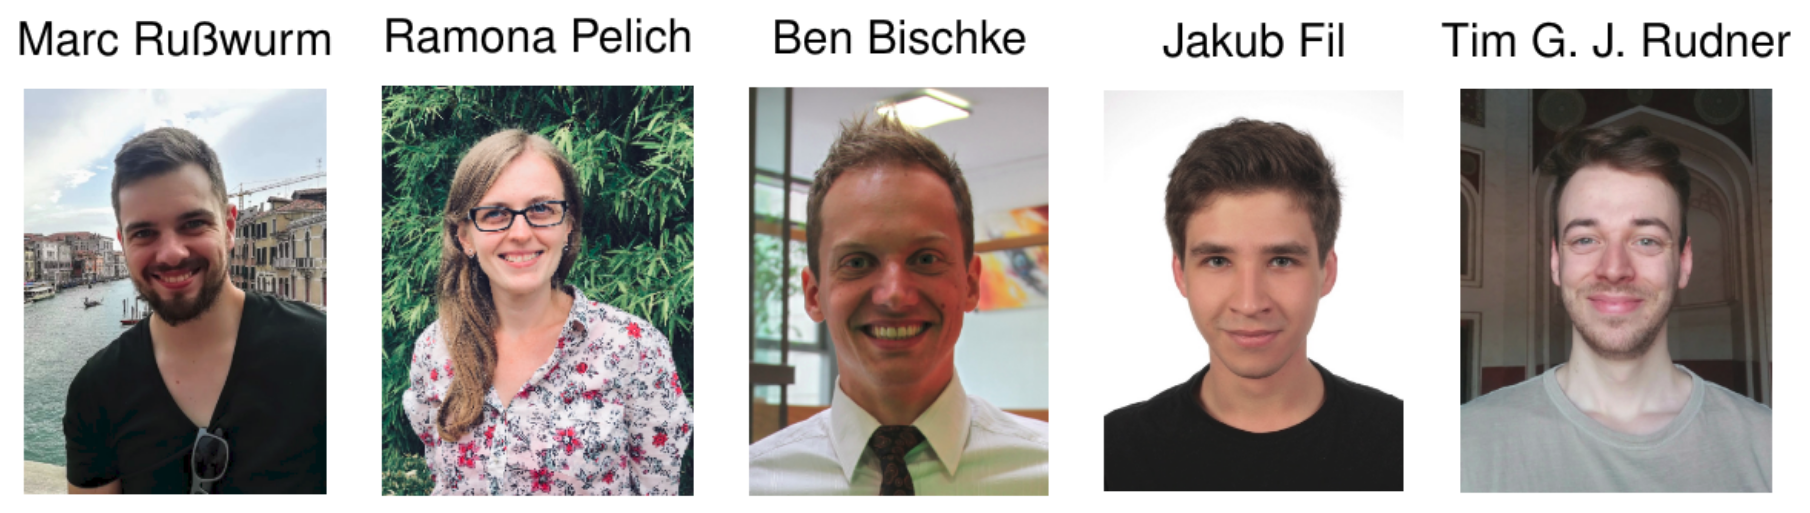
\includegraphics[height=3.5cm]{images/TheTeam}};
\node[right=.2em of team, inner sep=0](mentors){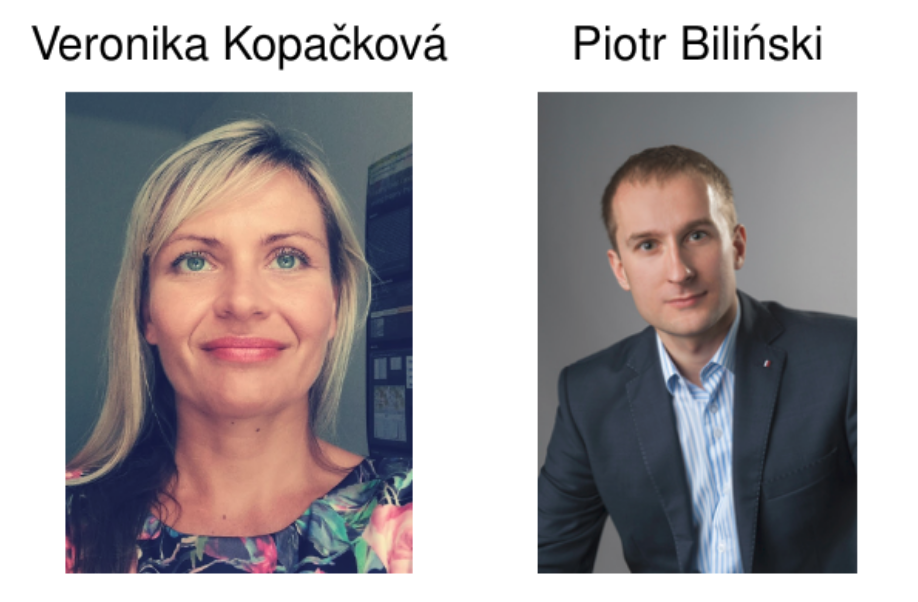
\includegraphics[height=3.5cm]{images/mentors}};
\end{tikzpicture}
\end{minipage}
\hspace{2em}
\begin{minipage}{0.6\linewidth}
%	\vspace{-1em}
	\figFusionNetwork

\end{minipage}

%\vspace{1em}
\section{Dense Time series for Vegetation Monitoring with Recurrent Networks}

\newcommand{\drawcbar}[5]{
	\def\tnode{#1} % iGate0
	\def\cmap{#2} % inferno
	\def\cbarheight{#3} % 1cm
	%	\def\vmin{#4} % 0
	%	\def\vmax{#5} % 1
	
	\node[right=1mm of \tnode, inner sep=0] (cbar\tnode){\includegraphics[height=4mm, width=\cbarheight, angle=90,origin=c]{\cmap}};
	\node[anchor=south, inner sep=0, xshift=5mm] at (cbar\tnode.south east) {\tiny #4};
	\node[anchor=north, inner sep=0, xshift=5mm] at (cbar\tnode.north east) {\tiny #5};
}
\newcommand{\imagecolumns}[2]{
		\foreach \t in {#1,...,#2}{
			\node[inner sep=0](times) at (\thetcounter*\hdist,-15mm){$t_{\the\numexpr\t+1\relax}$};
			\node[activation](xlast) at (\thetcounter*\hdist,-1*\vdist){\includegraphics[width=\imagewidth]{\folder/sample\s/time\t_x}};
			
%			\node[activation](flast1) at (\thetcounter*\hdist,-2*\vdist){\includegraphics[width=\imagewidth]{\folder/sample\s/time\t/\done_fGate}};
			\node[activation](clast3) at (\thetcounter*\hdist,-2*\vdist){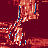
\includegraphics[width=\imagewidth]{\folder/sample\s/time\t/3_state}};
%			\node[activation](jlast1) at (\thetcounter*\hdist,-4*\vdist){\includegraphics[width=\imagewidth]{\folder/sample\s/time\t/\done_jGate}};
			\node[activation](clast22) at (\thetcounter*\hdist,-3*\vdist){
\includegraphics[width=\imagewidth]{\folder/sample\s/time\t/22_state}};
			\node[activation](clast1) at (\thetcounter*\hdist,-4.5*\vdist){\includegraphics[width=\imagewidth]{\folder/sample\s/time\t/\done_state}};
			\node[activation](ilast1) at (\thetcounter*\hdist,-5.5*\vdist){\includegraphics[width=\imagewidth]{\folder/sample\s/time\t/\done_iGate}};
			
			\stepcounter{tcounter}
		}
	}
	
	
\newcommand{\dotscolumn}{
	\node[activation] at (\thetcounter*\hdist,-1.5*\vdist){$\dots$};
	
	\node[activation,yshift=-1mm] at (\thetcounter*\hdist,-2.5*\vdist){$\dots$};
	\node[activation,yshift=-1mm] at (\thetcounter*\hdist,-3.5*\vdist){$\dots$};
	\node[activation,yshift=-1mm] at (\thetcounter*\hdist,-5*\vdist){$\dots$};
	\node[activation,yshift=-1mm] at (\thetcounter*\hdist,-6*\vdist){$\dots$};
	\stepcounter{tcounter}
}


\newcommand{\figactivations}[1]{
	% 1: number of sample
	% 2. number of activation
	
	\setcounter{tcounter}{0}
	
	\begin{tikzpicture}
	%\figGates{0}{18}{1}{3}
	\def\folder{images/activations/48px}
	
	\tikzstyle{activation}=[]
	\def\s{1}
	
	\def\done{#1}
	
	%% grid distance vertical and horizontal
	\def\vdist{22mm}
	\def\hdist{22mm}
	
	\def\imagewidth{21mm}
	
	%% descriptions top row
	\node[anchor=west] at (-1.7*\hdist,-1.8*\vdist){$\V{x}$};
%	\node[anchor=west](f1) at (-1.5*\hdist,-2.5*\vdist){$\V{f}^{(\done)}$};
	\node[anchor=west](i1) at (-1.7*\hdist,-2.7*\vdist){$\V{c}^{(3)}$};
%	\node[anchor=west](j1) at (-1.5*\hdist,-4.5*\vdist){$\V{j}^{(\done)}$};
	\node[anchor=west](c1) at (-1.7*\hdist,-3.7*\vdist){$\V{c}^{(22)}$};
	\node[anchor=west](c1) at (-1.7*\hdist,-5.2*\vdist){$\V{c}^{(47)}$};
	\node[anchor=west](c1) at (-1.7*\hdist,-6.2*\vdist){$\V{i}^{(47)}$};
	
	\imagecolumns{0}{1}
	\dotscolumn
	\imagecolumns{9}{20}
	\dotscolumn
	\imagecolumns{28}{30}
	
%	\drawcbar{flast1}{images/activations/inferno}{\imagewidth}{0}{1}
	\drawcbar{ilast1}{images/activations/inferno}{\imagewidth}{0}{1}
%	\drawcbar{jlast1}{images/activations/RdBu_r}{\imagewidth}{-1}{1}
	\drawcbar{clast1}{images/activations/RdBu_r}{\imagewidth}{-1}{1}
	\drawcbar{clast3}{images/activations/RdBu_r}{\imagewidth}{-1}{1}
	\drawcbar{clast22}{images/activations/RdBu_r}{\imagewidth}{-1}{1}
	
	\end{tikzpicture}
}
\newcounter{tcounter}
%\tikzsetnextfilename{network}

%\tikzstyle{operator} = [draw, circle, fill=tumbluemedium, draw=tumbluemedium, inner sep=0, text=white]
%\tikzstyle{function} = [draw, rectangle, fill=tumbluemedium, draw=tumbluemedium, text=white]
%\tikzstyle{gate} = [fill=tumivory,draw,rounded corners]

%\tikzstyle{dummy} = [inner sep=0]
\tikzstyle{flow} = [rounded corners, semithick]
\tikzstyle{endflow} = [-stealth,flow]
\tikzstyle{beginflow} = [stealth-,flow]
%\tikzstyle{perspective3drnn}=[z={(0.5cm,-0.5cm)}, x={(1cm,0cm)}, y={(0cm,1cm)}]
\tikzstyle{perspective3drnn}=[
x={(0.5cm,0.5cm)}, y={(1cm,0cm)}, z={(0cm,1cm)}]


\tikzstyle{bigpassbox} = [opacity=.2, rounded corners, draw=none]

\colorlet{forwardcolor}{focusone}%tumbluemedium
\colorlet{backwardcolor}{focustwo}
\colorlet{classcolor}{tumivory}

% defaultvalue -> might be replaced later
\colorlet{tensorcolor}{forwardcolor}

\tikzstyle{bigbox} = [rectangle, draw=tumivory, thick, fill=tumblack!20, rounded corners, 
inner sep=.5ex]

\tikzstyle{wireframe} = [draw=tumgray]


\tikzstyle{image} = [inner sep=0, fill=none, minimum size=\imagewidth]

\tikzset{pic shift/.store in=\shiftcoord,
	pic shift={(0,0)},
	pics/seqlstmfw/.style={
		code={
		\begin{scope}[shift={\shiftcoord},xscale=3,yscale=2]
			
			\node[dummy] (bl) at (0,0){}; % bottom left
			\node[dummy] (tr) at (1,1){}; % top right
			
			\node[dummy] (br) at ($ (bl -| tr) $){}; % bottom right
			\node[dummy] (tl) at ($ (bl |- tr) $){}; % top left
			
			\node[fit=(bl) (tr),bigbox] (-C) {};
			
			% input coordinate for rounded draw lines -> slightly right of tl
			\coordinate (-input) at (0.1,1); % top left
			
			% output coordinate for rounded draw lines -> slightly left of br
			\coordinate (-coutput) at (0.9,0); % bottom right
			\coordinate (-cinput) at (0.1,0); % bottom left
			\coordinate (-houtput) at (0.9,1); % bottom right
			
%			% gate distance
			\def\d{1/6}
			
			% gate heights
			\def\h{1/3}
			
			\coordinate (f)  at bl+(1*\d,0);
			\coordinate (i)  at bl+(2*\d,0);
			\coordinate (j)  at bl+(3*\d,0);
			\coordinate (o)  at bl+(4*\d,0);
			\coordinate (out) at bl+(5*\d,0);
			
			\coordinate (gates) at (0,2*\h);
			
			%\node[above=of tl](xt){$x_{t}$};
			%\node[left=of tl](htminus1){$h_{t-1}$};
			
			%\node[below=of br](ct){$c_{t}$};
			
			\node[inner sep=0](fgate) at ($ (gates -| f) $){};
			\node[inner sep=0](igate) at ($ (gates -| i) $){};
			\node[inner sep=0](jgate) at ($ (gates -| j) $){};
			\node[inner sep=0](ogate) at ($ (gates -| o) $){};
			
%			\coordinate (htminus1) at bl+(-.5,0);
%			\coordinate (ht) at bl+(-.5,0);
%			
			% forget gate
			\node[operator](fmult) at ($ (bl -| fgate) $) {};
			\draw[endflow] (-input) -| (fgate) -- (fmult); 
			
%			%j
			\node[operator](jmult) at ([shift={(0,-1*\h)}]jgate) {};
			\node[operator](cadd) at ($ (bl -| jgate) $) {};
			\draw[endflow] (-input) -| (jgate) -- (jmult);
			\draw[endflow] (jmult) -- (cadd); 			

%			%i	
			\draw[endflow] (-input) -| (igate) |- (jmult); 
%
%%			% outpu
			\node[operator](outtanh) at ([shift={(0,1*\h)}]out) {};
%			
%			%o 
			\draw[endflow] (tl) -| (ogate) |- (outtanh);
			\draw[flow] (outtanh) |- (-houtput);
%			
%			% output flow
			\draw[endflow] (cadd) -| (outtanh);
			\draw[flow] (-cinput) -- (fmult) -- (cadd) -- (-coutput);
%			
		\end{scope}
		}
	}
}

\tikzset{pic shift/.store in=\shiftcoord,
	pic shift={(0,0)},
	pics/seqlstmbw/.style={
		code={
			\begin{scope}[shift={\shiftcoord},xscale=3,yscale=-2]
				
				\node[dummy] (bl) at (0,0){}; % bottom left
				\node[dummy] (tr) at (1,1){}; % top right
				
				\node[dummy] (br) at ($ (bl -| tr) $){}; % bottom right
				\node[dummy] (tl) at ($ (bl |- tr) $){}; % top left
				
				\node[fit=(bl) (tr),bigbox] (-C) {};
				
				% input coordinate for rounded draw lines -> slightly right of tl
				\coordinate (-input) at (0.1,1); % top left
				
				% output coordinate for rounded draw lines -> slightly left of br
				\coordinate (-coutput) at (0.9,0); % bottom right
				\coordinate (-cinput) at (0.1,0); % bottom left
				\coordinate (-houtput) at (0.9,1); % top right
				
				%			% gate distance
				\def\d{1/6}
				
				% gate heights
				\def\h{1/3}
				
				\coordinate (f)  at bl+(1*\d,0);
				\coordinate (i)  at bl+(2*\d,0);
				\coordinate (j)  at bl+(3*\d,0);
				\coordinate (o)  at bl+(4*\d,0);
				\coordinate (out) at bl+(5*\d,0);
				
				\coordinate (gates) at (0,2*\h);
				
				%\node[above=of tl](xt){$x_{t}$};
				%\node[left=of tl](htminus1){$h_{t-1}$};
				
				%\node[below=of br](ct){$c_{t}$};
				
				\node[inner sep=0](fgate) at ($ (gates -| f) $){};
				\node[inner sep=0](igate) at ($ (gates -| i) $){};
				\node[inner sep=0](jgate) at ($ (gates -| j) $){};
				\node[inner sep=0](ogate) at ($ (gates -| o) $){};
				
				%			\coordinate (htminus1) at bl+(-.5,0);
				%			\coordinate (ht) at bl+(-.5,0);
				%			
				% forget gate
				\node[operator](fmult) at ($ (bl -| fgate) $) {};
				\draw[endflow] (-input) -| (fgate) -- (fmult); 
				
				%			%j
				\node[operator](jmult) at ([shift={(0,-1*\h)}]jgate) {};
				\node[operator](cadd) at ($ (bl -| jgate) $) {};
				\draw[endflow] (-input) -| (jgate) -- (jmult);
				\draw[endflow] (jmult) -- (cadd); 			
				
				%			%i	
				\draw[endflow] (-input) -| (igate) |- (jmult); 
				%
				%%			% outpu
				\node[operator](outtanh) at ([shift={(0,1*\h)}]out) {};
				%			
				%			%o 
				\draw[endflow] (tl) -| (ogate) |- (outtanh);
				\draw[flow] (outtanh) |- (-houtput);
				%			
				%			% output flow
				\draw[endflow] (cadd) -| (outtanh);
				\draw[flow] (-cinput) -- (fmult) -- (cadd) -- (-coutput);
				
			\end{scope}
		}
	}
}

\newcommand{\tensorcube}[4]{
	\def\w{#1}
	\def\h{#2}
	\def\d{#3}
	\def\img{#4}
	
	\begin{scope}[perspective3drnn]
		
		% bw back frame
		\begin{scope}[canvas is yz plane at x=\d]
			\node[transform shape,image, minimum size=\w, anchor=south west, fill=none, wireframe](back){};
		\end{scope}
		
		% front image
		\begin{scope}[canvas is yz plane at x=0]
			\node[transform shape,image, anchor=south west, opacity=1](front){\includegraphics[width=\w]{\img}};
		\end{scope}
		
		% front frame
		\begin{scope}[canvas is yz plane at x=0]
			\node[transform shape,image, minimum size=\w, anchor=south west, fill=none, wireframe](front){};
		\end{scope}
		
		% fill right side
		\fill[tensorcolor,opacity=.5, wireframe] (front.south east) -- (back.south east) -- (back.north east) -- (front.north east);
		% fill top side
		\fill[tensorcolor,opacity=.5,opacity=0.6, wireframe] (front.north east) -- (back.north east) -- (back.north west) -- (front.north west);
		% fill right side
		
		
		%\draw[] (front.south west) -- (back.south west);
		
	\end{scope}
}

\newcommand{\concatstates}[4]{
	\def\w{#1}
	\def\h{#2}
	\def\d{#3}
	\def\img{#4}
	
	\begin{scope}[perspective3drnn]
		
		% bw back frame
		\begin{scope}[canvas is yz plane at x=2*\d]
			\node[transform shape,image, minimum size=\w, anchor=south west, fill=none, wireframe](back){};
		\end{scope}
		
		% middle frame
		\begin{scope}[canvas is yz plane at x=\d]
			\node[transform shape,image, minimum size=\w, anchor=south west, fill=none, wireframe](middle){};
		\end{scope}
		
		% front image
		\begin{scope}[canvas is yz plane at x=0]
			\node[transform shape,image, anchor=south west](front){\includegraphics[width=\w]{\img}};
		\end{scope}
		
		% front frame
		\begin{scope}[canvas is yz plane at x=0]
			\node[transform shape,image, minimum size=\w, anchor=south west, fill=none,wireframe](front){};
		\end{scope}
		
		% fill right side
		\fill[backwardcolor,opacity=.5, wireframe] (front.south east) -- (middle.south east) -- (middle.north east) -- (front.north east);
		% fill top side
		\fill[backwardcolor,opacity=.5,opacity=0.6, wireframe] (front.north east) -- (middle.north east) -- (middle.north west) -- (front.north west);
		% fill right side
		
		\fill[forwardcolor,opacity=.5, wireframe] (middle.south east) -- (back.south east) -- (back.north east) -- (middle.north east);
		% fill top side
		\fill[forwardcolor,opacity=.5,opacity=0.6, wireframe] (middle.north east) -- (back.north east) -- (back.north west) -- (middle.north west);
		
		%\draw[] (front.south west) -- (back.south west);
		
		
	\end{scope}
}

\newcommand{\figseqencnetwork}{
\begin{tikzpicture}[scale=1, node distance=1em]
%
\def\d{4.2}%
\def\encoderheight{1}%
\def\decoderheight{-1}%
\def\imagewidth{30mm}%
\def\stateimagewidth{30mm}%
\def\classimagewidth{40mm}%
%
\def\rgbone{images/seqencnetwork/rgb1}%
\def\rgbtwo{images/seqencnetwork/rgb2}%
\def\rgbthree{images/seqencnetwork/rgb3}%
\def\rgbfour{images/seqencnetwork/rgb4}%
\def\prediction{images/seqencnetwork/prediction}%
\def\groundtruth{images/seqencnetwork/ground_truth}%
\def\activation{images/seqencnetwork/maize}%
\def\state{images/seqencnetwork/state}%
%
\draw pic (fw1) at (\d,\encoderheight) {seqlstmfw};% \&
\node[above=of fw1tl, inner sep=0](xfw1){\includegraphics[width=\imagewidth]{\rgbone}};%images/network/time1_x
\node[above=0em of xfw1, inner sep=0](labxfw1){$\V{x}_{0}$};

\draw pic (fw2) at (2*\d,\encoderheight) {seqlstmfw};
\node[above=of fw2-input, inner sep=0](xfw2){\includegraphics[width=\imagewidth]{\rgbtwo}}; % images/network/time11_x
\node[above=0em of xfw2, inner sep=0](labxfw2){$\V{x}_{1}$};

\draw pic (fw3) at (3*\d,\encoderheight) {seqlstmfw};
\node[above=1em of fw3-input](xfw3){$\dots$};

\draw pic (fw4) at (4*\d,\encoderheight) {seqlstmfw};
\node[above=of fw4-input, inner sep=0](xfw4){\includegraphics[width=\imagewidth]{\rgbfour}}; % images/network/time30_x
\node[above=0em of xfw4, inner sep=0](labxfw4){$\V{x}_T$};

\node[left=of fw1-input](enczerostateh){$\V{h}_0 = \V{0}$};
\node[left=of fw1-cinput](enczerostatec){$\V{c}_0 = \V{0}$};

\draw[endflow] (enczerostateh) -- (fw1-input);
\draw[endflow] (enczerostatec) -- (fw1-cinput);

% draw connections from input to cells
\draw[flow] (xfw1) |- (fw1-input);
\draw[flow] (xfw2) |- (fw2-input);
\draw[flow] (xfw3) |- (fw3-input);
\draw[flow] (xfw4) |- (fw4-input);

% draw hidden connections between cells
\draw[endflow] (fw1-houtput) -- (fw2-input);
\draw[endflow] (fw2-houtput) -- (fw3-input);
\draw[endflow] (fw3-houtput) -- (fw4-input);

% draw hidden connections between cells
\draw[endflow] (fw1-coutput) -- (fw2-cinput);
\draw[endflow] (fw2-coutput) -- (fw3-cinput);
\draw[endflow] (fw3-coutput) -- (fw4-cinput);

\coordinate[right=of fw4-coutput](rightend);

%\node(concatstates) at (6.2*\d,0){
\node[above right= 0em and 2em of fw4-coutput](concatstates){
\begin{tikzpicture}
\concatstates{\stateimagewidth}{\stateimagewidth}{2}{\state}
\end{tikzpicture}
};
\node[above=0em of concatstates, inner sep=0](labct){$\V{c}_T$};

\draw[endflow] (fw4-coutput) -- ++(.2em,0) |- (concatstates);
%\draw[endflow] (cbw) -- (concatstates);

%\path[draw] (0,0) -- (0,1) -- (1,1) -- (1,0) -- (0,0);

\node[right=of concatstates](conv){
	\begin{tikzpicture}
	    \colorlet{tensorcolor}{classcolor}
		\tensorcube{\stateimagewidth}{\stateimagewidth}{.75}{\activation} %images/network/48px/72_state
	\end{tikzpicture}
};

\node[rectangle, minimum width=4mm, minimum height=4mm, fill=tumblue, draw=tumblue, opacity=1, rounded corners=0, semithick](inconvrect) at ($ (concatstates) + (-3mm,-3mm) $){};
%\node[below=0mm of inconvrect](){\tiny \color{white} $\kclass$};

\node[rectangle, minimum width=2mm, minimum height=2mm, fill=tumblue, draw=tumblue, opacity=1, inner sep=0, semithick, rounded corners=0](outconvrect) at (conv){};

\draw[tumblue, semithick, rounded corners=0, fill=tumbluedark, opacity=.5] (inconvrect.north east) -- (outconvrect.north west) -- (outconvrect.south west) -- (inconvrect.south east);

\coordinate(convcenter) at ($ (inconvrect)!0.5!(outconvrect) $);

\node[right=of conv](pred){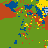
\includegraphics[width=\classimagewidth]{\prediction}}; %$\hat{\V{y}}$
%\node[above right=of conv, label={north:label}](ground){\includegraphics[width=\classimagewidth]{\groundtruth}}; % $\V{y}}$

\draw[endflow] (conv) -- (pred); % node[midway, right] {\small argmax}; 
%\draw[<->] (ground) -- (conv) node[midway, right] {\small $H(\V{y},\hat{\V{y}})$};

\coordinate(cltop) at (concatstates |- labxfw4);

\node[below= 3.5em of fw1-input, xshift=1em, noteannot, draw=none](annotlstm){%
	\textbf{long short-term memory cell} \\ 
	sequentially processes \\ 
	data keeping long-term \\ 
	and short-term memory \\
	\\
	%	hidden state $\V{h}$ as short-, \\
	%	cell state $\V{c}$ as long-term memory; both initialized as $\V{0}$ \\
	\verytiny\baselineskip=5pt Hochreiter, S., \& Schmidhuber, J. \\ \verytiny\baselineskip=5pt (1997). \textbf{Long short-term memory}. \\ \verytiny\baselineskip=5pt Neural computation, 9(8), 1735-1780.\par
};

\node[right=-2em of annotlstm, yshift=0em](lstmcell){\figlstmexplain};

\begin{scope}[on background layer]
	\node[fill=focusone!10, rounded corners, fit=(enczerostatec)(labxfw1)(labxfw4)(rightend), inner sep=.2em]{};
	\node[fill=focustwo!10, rounded corners, fit=(concatstates)(conv)(labct)(cltop), inner sep=.2em]{};
	\node[fit=(lstmcell)(annotlstm), rounded corners, inner sep=0, noteannot](boxlstm){};
	
\end{scope}



\draw[annotation] (boxlstm) -- (fw1jmult);
\draw[annotation] (boxlstm) -- (fw2jmult);
\draw[annotation] (boxlstm) -- (fw3jmult);
\draw[annotation] (boxlstm) -- (fw4jmult);

%\node[below= 4em of fw1-input, noteannot](annothidden){\textbf{hidden cell output} $\V{h}_t$ \\ stores short-term memory};
%\node[below= of annothidden, noteannot](annotstate){\textbf{cell state} $\V{c}_t$ \\ stores long-term memory};

\node[above=3.5em of outconvrect, xshift=1em, noteannot](annotconv){\textbf{convolution} \textbf{and softmax} compresses the \\ dimensionality to the number of classes};
\draw[annotation] (annotconv) -- (convcenter);

\node[below=2em of conv, xshift=-3em, noteannot](annotactivations){\textbf{output activations} \\ as confidences \\ for each class};
\draw[annotation](annotactivations) -- (conv);

\node[below=1.5em of pred, xshift=1em, noteannot](annotprediction){\textbf{prediction} as \\ class of highest \\ activation};
\draw[annotation](annotprediction) -- (pred);

\node[above=1.5em of xfw2, xshift=1em, noteannot](annotx){\textbf{input sequence} of Sentinel 2 images};
\draw[annotation] (annotx) -- (xfw1);
\draw[annotation] (annotx) -- (xfw2);
\draw[annotation] (annotx) -- (xfw4);

\begin{scope}[node distance=.5em]
\node[inner sep=0, label={below:\tiny maize}, below= 1.2em of annotactivations, xshift=-2em](a){
\includegraphics[width=3cm]{images/examples/16494/maize}};
\node[inner sep=0, label={below:\tiny meadow}, right=of a](b){
\includegraphics[width=3cm]{images/examples/16494/meadow}};
\node[inner sep=0, label={below:\tiny wheat}, right=of b](c){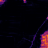
\includegraphics[width=3cm]{images/examples/16494/winter_wheat}};
\node[inner sep=0, label={below:\tiny peas}, right=of c](d){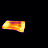
\includegraphics[width=3cm]{images/examples/16494/peas}};
\node[inner sep=0, label={below:\tiny rapeseed}, right=of d](e){
\includegraphics[width=3cm]{images/examples/16494/rape}};
\end{scope}

\draw[annotation] (annotactivations) -- (c);


\node[below=2em of annotlstm, xshift=15.5cm](actnormal){\figactivations{47}};


\node[noteannot, above= 0em of actnormal, xshift=5em](a){\textbf{cells extract features} sequentially from the input data};
\draw[annotation] (a)++(5em,-1em) -- ++(2em,-5em);
\draw[annotation] (a)++(5em,-1em) -- ++(2em,-7em);

\node[noteannot, below= .5em of actnormal, xshift=-5em](b){\textbf{cells mask clouds} indicated by the input gate $\V{i}$ closing (values of zero)};
\draw[annotation] (b) -- ++(-4em,2em);
\draw[annotation] (b) -- ++(10em,2em);
\draw[annotation] (b) -- ++(21em,2em);

\node[left=3em of a]{LSTM cell activations:};
\end{tikzpicture}
}

\begin{minipage}{0.35\linewidth} 
\textbf{Recurrent Neural Networks} \\ learn patterns in sequential data.

\vspace{-.5em}
\subsection{Application}
We insert a \pre{sequence of satellite images} to learn \textbf{vegetation life cycle} events for field crop identification.

\subsection{Automatic Cloud Filtering}
Area of interest covered by clouds.

\usepgfplotslibrary{groupplots}

%\tikzsetnextfilename{scl}
\begin{tikzpicture}

%\def\data{images/classhist/classHistograms.dat}
\def\data{images/clouds/scl2.csv}

\pgfplotsset{ every non boxed x axis/.append style={x axis line style=-},
	every non boxed y axis/.append style={y axis line style=-}}

\pgfplotsset{every axis/.append style={ybar=1pt, bar width=6pt, ymajorgrids}}
\pgfplotsset{every axis label/.append style={font=\footnotesize},tick pos=left,ylabel near ticks}
\pgfplotsset{every x tick label/.append style={rotate=90,anchor=east,font=\fontsize{9}{9}\selectfont}}
%   \pgfplotsset{every y tick label/.append style={/pgf/number format/.cd, fixed, precision=2, fixed zerofill,}}
%\tikzstyle{caption}=[font=\footnotesize, fill=tumwhite, fill opacity=.5, text opacity=1]


\begin{axis}[
%group style={
%	%       group size=1 by 4,
%	group size=1 by 1,
%	xlabels at=edge bottom,
%	xticklabels at=edge bottom,
%	ylabels at=edge left,
%	yticklabels at=edge left,
%	vertical sep=2pt,
%	horizontal sep=2pt
%},
width=.9\textwidth,
height=6cm,
%ymode=log,
%log origin=infty,
%     y dir=reverse,
%     scaled ticks=true,
%log ticks with fixed point,
%scaled x ticks=true,
axis lines=left,
xlabel={}, % image acquisition dates
ylabel={},
title={\small cloud coverage per observation},
xlabel style={yshift=2mm},
xmin=-.5,
xmax=46,
%xlabel=clouds,
ytick={1,10,25,50,100},
yticklabels={\SI{1}{\percent},\SI{10}{\percent},\SI{25}{\percent},\SI{50}{\percent},\SI{100}{\percent}},
xtick=data,
xticklabels={
	03. Jan,
	13. Jan,
	20. Jan,
	21. Jan,
	28. Jan,
	12. Feb,
	11. Mär,
	20. Mär,
	23. Mär,
	03. Apr,
	13. Apr,
	19. Apr,
	22. Apr,
	29. Apr,
	02. Mai,
	10. Mai,
	22. Mai,
	29. Mai,
	08. Jun,
	18. Jun,
	28. Jan,
	02. Jul,
	14. Jul,
	18. Jul,
	21. Jul,
	28. Jul,
	30. Jul,
	07. Aug,
	17. Aug,
	20. Aug,
	28. Aug,
	21. Aug,
	09. Sep,
	12. Sep,
	18. Sep,
	26. Sep,
	29. Sep,
	09. Okt,
	18. Okt,
	28. Okt,
	09. Nov,
	15. Nov,
	18. Nov,
	28. Nov,
	06. Dez,
	08. Dez
},
axis on top
];

\addplot[
%       draw=tumblue,
draw=none,
fill=tumblue,rounded corners=.5pt
] table [col sep=comma, x=id, y=cloudpercent] {\data};


\end{axis}
\end{tikzpicture}

%\vspace{.2em}
We \textbf{trained} the network on \textbf{cloudy} and \textbf{non-cloudy} datasets.
%usepgfplotslibrary{fillbetween}

%\newcommand{\fbopacity}{0.3}
%\newcommand{\skippoints}{2}


%\def\measure{oa}
\def\height{3.5cm}


%\colorlet{L1Ccolor}{tumblue}
%colorlet{L2Acolor}{tumblack}

%\colorlet{clouds01color}{tumred}
%\colorlet{clouds10color}{tumorange}
%\colorlet{clouds25color}{tumgray}
%\colorlet{clouds50color}{tumblue}
%\colorlet{clouds80color}{tumblack}

\colorlet{clouds01color}{tumbluedark!55}
\colorlet{clouds10color}{tumbluedark!70}
\colorlet{clouds25color}{tumbluedark!85}
\colorlet{clouds50color}{tumbluedark}
\colorlet{clouds80color}{tumblack}

\colorlet{highlightcolor}{tumgraylight!25}

%\colorlet{2017traincolor}{tumgray}
%\colorlet{2017testcolor}{tumblack}

\tikzset{new spy style/.style={spy scope={%
			magnification=2,
			connect spies,
			every spy on node/.style={
				rectangle,
				rounded corners=1pt,
				draw,
			},
			every spy in node/.style={
				draw,
				rectangle,
				rounded corners=1pt,
				fill=gray!40,
			}
		}
	}
} 


%\tikzsetnextfilename{clouds}
\begin{tikzpicture}[new spy style, remember picture]
	
	% replaced by global settings in figures.tex
	\pgfplotsset{every axis plot/.append style={line width=2pt}}
	
	
	\begin{groupplot}[
	group style={
		group size=2 by 1,
		xlabels at=edge bottom,
		ylabels at=edge left,
		xticklabels at=edge bottom,
		vertical sep=35pt,
		group name=trainplot
	},
	legend style={
		at={(.75,0)},
		title=test,
		anchor=south,
		fill=tumgraylight!50,
		rounded corners=1pt,
		draw=none,
		font=\veryverytiny, 
		legend image post style={line width =5pt},
		/tikz/every even column/.append style={column sep=0.2cm},
	},
	axis lines=left,
	grid=both,
	scaled x ticks = false,
%	y tick label style={/pgf/number format/fixed},
	grid style={draw=tumgraylight},
	legend columns=2,
	width=.9\textwidth,
	height=6cm,
	xlabel={\tiny samples seen},
	xlabel style={yshift=-4mm},
	xtick={200000,300000,400000,500000,600000,700000,800000,900000,1000000},
	xticklabels={200k,300k,400k,500k,600k,700k,800k,900k,1000k},
	xmin=100000,
	xmax=800000,
	ymin=.85,
	ymax=.95]


\nextgroupplot[title={\small overall pixel accuracy over training},ymin=.75,ymax=.94]
\pgfplotsset{every x tick label/.append style={font=\verytiny\selectfont}}

\coordinate (topsource) at (axis cs: 800000,.96);
\coordinate (bottomsource) at (axis cs: 800000,.84);

\coordinate (topsourceleft) at (axis cs: 0,.96);
\coordinate (bottomsourceleft) at (axis cs: 0,.84);

%\fill[highlightcolor,draw=tumgraylight, rounded corners=1pt] (bottomsource) -- (bottomsourceleft) -- (topsourceleft) -- (topsource); 

\addplot[clouds01color, forget plot] table [x=Step, y = clouds01_test2016clouds01_oa, col sep=comma] {images/clouds/train_rw15.csv};

\addplot[clouds10color, forget plot] table [x=Step, y = clouds10_test2016clouds10_oa, col sep=comma] {images/clouds/train_rw15.csv};

\addplot[clouds25color, forget plot] table [x=Step, y = clouds25_test2016clouds25_oa, col sep=comma] {images/clouds/train_rw15.csv};

\addplot[clouds50color, forget plot] table [x=Step, y = clouds50_test2016clouds50_oa, col sep=comma] {images/clouds/train_rw15.csv};

\addplot[clouds80color, forget plot] table [x=Step, y = clouds80_test2016_oa, col sep=comma] {images/clouds/train_rw15.csv};



%\nextgroupplot[
%	title=,
%	ylabel={ov. acc.}, 
%	ymin=.84,
%	ymax=.96, 
%	xmin=0,
%	axis y line*=right,
%	ylabel near ticks, 
%	yticklabel pos=right,
%	grid=both,
%	grid style={tumgray!50},
%	axis background/.style={fill=highlightcolor},
%	]
%\addplot[clouds01color] table [x=Step, y = clouds01_test2016clouds01_oa, col sep=comma] {images/clouds/train_rw15.csv};

\addlegendentry{$<$ \SI{1}{\percent} (4 obs.)}

\addplot[clouds10color] table [x=Step, y = clouds10_test2016clouds10_oa, col sep=comma] {images/clouds/train_rw15.csv};
\addlegendentry{$<$ \SI{10}{\percent} (10 obs.)}

\addplot[clouds25color] table [x=Step, y = clouds25_test2016clouds25_oa, col sep=comma] {images/clouds/train_rw15.csv};
\addlegendentry{$<$ \SI{25}{\percent} (17 obs.)}

\addplot[clouds50color] table [x=Step, y = clouds50_test2016clouds50_oa, col sep=comma] {images/clouds/train_rw15.csv};
\addlegendentry{$<$ \SI{50}{\percent} (23 obs.)}

\addplot[clouds80color] table [x=Step, y = clouds80_test2016_oa, col sep=comma] {images/clouds/train_rw15.csv};
\addlegendentry{all images (46 obs.)}

\node [above,font=\verytiny, inner sep=2pt] (LT) at (rel axis cs: .68,.35) {cloud coverage less than:};

\coordinate (toptarget) at (rel axis cs: 0,1);
\coordinate (bottomtarget) at (rel axis cs: 0,0);

\end{groupplot}

%\draw[fill=highlightcolor, draw=tumgraylight] (topsource) -- (toptarget) -- (bottomtarget)  -- (bottomsource);
%\draw[|-|, tumgray] ($ (bottomsource) + (0ex,0) $) -- ($ (topsource) + (0ex,0) $);
%\draw[|-|, tumgray] (bottomtarget) -- (toptarget);

\end{tikzpicture}  

Similar accuracy on data with clouds, due to some cells having learned cloud masking from provided data.
	
\end{minipage}
\hspace{2em}
\begin{minipage}{0.6\linewidth}
%	\vspace{-2em}
	\figseqencnetwork
\end{minipage}


%\newcommand{\examplescenescbar}{
	\begin{tikzpicture}[inner sep=0]
	\node(cbar){
\includegraphics[height=\size, width=2mm]{images/examples/inferno}};
	\node[xshift=1mm, anchor=north] at (cbar.north east){\tiny 1};
	\node[xshift=1mm, anchor=south] at (cbar.south east){\tiny 0};
	\end{tikzpicture}
}


% for text extending below like p, q, g
%\tikzset{
%	mylabel2/.style={
%		label={
%			[label distance=-1.25em, anchor=base]north:
%			\fcolorbox{black}{black}{
%				\scriptsize \color{tumgraylight} #1
%			}
%		}
%	}
%}


\begin{tikzpicture}
\tikzset{
	collabel/.style={
		label={
			[label distance=1.5em, anchor=base]south:
			\tiny \color{black} #1
		}
	}
}

\setlength{\fboxsep}{1pt}
\tikzset{
	inlabel/.style={
		label={
			[label distance=-1em, anchor=base]north:
			\fcolorbox{black}{black}{
				\scriptsize \color{tumgraylight} #1
			}
		}
	}
}

\tikzset{
	rowlabel/.style={
		label={
			[label distance=.51em, anchor=north west]north west:
			\fcolorbox{white}{white}{
				\color{black} \textbf{#1}
			}
		}
	}
}

\def\size{1.7cm}
\def\colsize{7mm}

\colsize
\small

\matrix (m) [matrix of nodes, ampersand replacement=\&, row sep=0pt, column sep=2mm]{
	$\V{x}_{RGB,t}$ \& labels $\V{y}$ \& pred. $\hat{\V{y}}$ \& loss $H(\V{y},\hat{\V{y}}$) \& activation \& activation \& activation \& activation
	\\ %% good classificaiton example
	\node[rowlabel=A,inner sep=0]{
\includegraphics[width=\size]{images/examples/16494/rgb}}; \&
	\node[inner sep=0]{\includegraphics[width=\size]{images/examples/16494/ground_truth}}; \&
	\node[inner sep=0]{\includegraphics[width=\size]{images/examples/16494/prediction}}; \&
	\node[inner sep=0]{\includegraphics[width=\size]{images/examples/16494/masked_loss}}; \&
	\node[inlabel=maize,inner sep=0]{\includegraphics[width=\size]{images/examples/16494/maize}}; \&
	\node[inlabel=meadow,inner sep=0]{\includegraphics[width=\size]{images/examples/16494/meadow}}; \&
	\node[inlabel=peas,inner sep=0]{\includegraphics[width=\size]{images/examples/16494/peas}}; \&
	\node[inlabel=rape,inner sep=0]{\includegraphics[width=\size]{images/examples/16494/rape}}; \&
	\examplescenescbar 
	\\ %% Good example with correct prediction, but some loss
	\node[rowlabel=B,inner sep=0]{\includegraphics[width=\size]{images/examples/8133/rgb}}; \&
	\node[inner sep=0]{\includegraphics[width=\size]{images/examples/8133/ground_truth}}; \&
	\node[inner sep=0]{\includegraphics[width=\size]{images/examples/8133/prediction}}; \&
	\node[inner sep=0]{\includegraphics[width=\size]{images/examples/8133/masked_loss}}; \&
	\node[inlabel=spelt,inner sep=0]{\includegraphics[width=\size]{images/examples/8133/winter_spelt}}; \&
	\node[inlabel=wheat,inner sep=0]{\includegraphics[width=\size]{images/examples/8133/winter_wheat}}; \&
	\node[inlabel=s. barley,inner sep=0]{\includegraphics[width=\size]{images/examples/8133/summer_barley}}; \&
	\node[inlabel=maize,inner sep=0]{\includegraphics[width=\size]{images/examples/8133/maize}}; \&
	\examplescenescbar 
	\\ %% Good example, only one small field partly wrong classified
	\node[rowlabel=C,inner sep=0]{\includegraphics[width=\size]{images/examples/1823/rgb}}; \&
	\node[inner sep=0]{\includegraphics[width=\size]{images/examples/1823/ground_truth}}; \&
	\node[inner sep=0]{\includegraphics[width=\size]{images/examples/1823/prediction}}; \&
	\node[inner sep=0]{\includegraphics[width=\size]{images/examples/1823/masked_loss}}; \&
	\node[inlabel=meadow,inner sep=0]{\includegraphics[width=\size]{images/examples/1823/meadow}}; \&
	\node[inlabel=wheat,inner sep=0]{\includegraphics[width=\size]{images/examples/1823/winter_wheat}}; \&
	\node[inlabel=oat,inner sep=0]{\includegraphics[width=\size]{images/examples/1823/summer_oat}}; \&
	\node[inlabel=maize,inner sep=0]{\includegraphics[width=\size]{images/examples/1823/maize}}; \&
	\examplescenescbar 
	\\ %% narrow fields
	\node[rowlabel=D,inner sep=0]{\includegraphics[width=\size]{images/examples/12894/rgb}}; \&
	\node[inner sep=0]{\includegraphics[width=\size]{images/examples/12894/ground_truth}}; \&
	\node[inner sep=0]{\includegraphics[width=\size]{images/examples/12894/prediction}}; \&
	\node[inner sep=0]{\includegraphics[width=\size]{images/examples/12894/masked_loss}}; \&
	\node[inlabel=meadow,inner sep=0]{\includegraphics[width=\size]{images/examples/12894/meadow}}; \&
	\node[inlabel=wheat,inner sep=0]{\includegraphics[width=\size]{images/examples/12894/winter_wheat}}; \&
	\node[inlabel=potato,inner sep=0]{\includegraphics[width=\size]{images/examples/12894/potatoe}}; \&
	\node[inlabel=maize,inner sep=0]{\includegraphics[width=\size]{images/examples/12894/maize}}; \&
	\examplescenescbar 
%	\\ %% Good example, only one small field partly wrong classified
%	\node[rowlabel=D,inner sep=0]{\includegraphics[width=\size]{images/examples/2550/rgb}}; \&
%	\node[inner sep=0]{\includegraphics[width=\size]{images/examples/2550/ground_truth}}; \&
%	\node[inner sep=0]{\includegraphics[width=\size]{images/examples/2550/prediction}}; \&
%	\node[inner sep=0]{\includegraphics[width=\size]{images/examples/2550/masked_loss}}; \&
%	\node[inlabel=maize,inner sep=0]{\includegraphics[width=\size]{images/examples/2550/maize}}; \&
%	\node[inlabel=wheat,inner sep=0]{\includegraphics[width=\size]{images/examples/2550/winter_wheat}}; \&
%	\node[inlabel=s. barley,inner sep=0]{\includegraphics[width=\size]{images/examples/2550/summer_barley}}; \&
%	\node[inlabel=w. barley,inner sep=0]{\includegraphics[width=\size]{images/examples/2550/winter_barley}}; \&
%	\examplescenescbar 
%	\\ %% Exampe of a forrest, which us a unknown class!
%	\node[rowlabel=D,inner sep=0]{\includegraphics[width=\size]{images/examples/2554/rgb}}; \&
%	\node[inner sep=0]{\includegraphics[width=\size]{images/examples/2554/ground_truth}}; \&
%	\node[inner sep=0]{\includegraphics[width=\size]{images/examples/2554/prediction}}; \&
%	\node[inner sep=0]{\includegraphics[width=\size]{images/examples/2554/masked_loss}}; \&
%	\node[inlabel=maize,inner sep=0]{\includegraphics[width=\size]{images/examples/2554/maize}}; \&
%	\node[inlabel=wheat,inner sep=0]{\includegraphics[width=\size]{images/examples/2554/winter_wheat}}; \&
%	\node[inlabel=meadow,inner sep=0]{\includegraphics[width=\size]{images/examples/2554/meadow}}; \&
%	\node[inlabel=w. barley,inner sep=0]{\includegraphics[width=\size]{images/examples/2554/winter_barley}}; \&
%	\examplescenescbar 
%	\\ %% sparse label feature map
%	\node[rowlabel=A,inner sep=0]{\includegraphics[width=\size]{images/examples/10791/rgb}}; \&
%	\node[inner sep=0]{\includegraphics[width=\size]{images/examples/10791/ground_truth}}; \&
%	\node[inner sep=0]{\includegraphics[width=\size]{images/examples/10791/prediction}}; \&
%	\node[inner sep=0]{\includegraphics[width=\size]{images/examples/10791/masked_loss}}; \&
%	\node[inlabel=maize,inner sep=0]{\includegraphics[width=\size]{images/examples/10791/maize}}; \&
%	\node[inlabel=wheat,inner sep=0]{\includegraphics[width=\size]{images/examples/10791/winter_wheat}}; \&
%	\node[inlabel=meadow,inner sep=0]{\includegraphics[width=\size]{images/examples/10791/meadow}}; \&
%	\node[inlabel=w. barley,inner sep=0]{\includegraphics[width=\size]{images/examples/10791/winter_barley}}; \&
%	\examplescenescbar 
	\\ %% one field completely wrong classified. one field uncertain
	\node[rowlabel=E,inner sep=0]{\includegraphics[width=\size]{images/examples/10792/rgb}}; \&
	\node[inner sep=0]{\includegraphics[width=\size]{images/examples/10792/ground_truth}}; \&
	\node[inner sep=0]{\includegraphics[width=\size]{images/examples/10792/prediction}}; \&
	\node[inner sep=0]{\includegraphics[width=\size]{images/examples/10792/masked_loss}}; \&
	\node[inlabel=rye,inner sep=0]{\includegraphics[width=\size]{images/examples/10792/winter_rye}}; \&
	\node[inlabel=wheat,inner sep=0]{\includegraphics[width=\size]{images/examples/10792/winter_wheat}}; \&
	\node[inlabel=triticale,inner sep=0]{\includegraphics[width=\size]{images/examples/10792/winter_triticale}}; \&
	\node[inlabel=s. barley,inner sep=0]{\includegraphics[width=\size]{images/examples/10792/summer_barley}}; \&
	\examplescenescbar 
	\\ %% Multiple fields uncertain
%	\node[rowlabel=A,inner sep=0]{\includegraphics[width=\size]{images/examples/10879/rgb}}; \&
%	\node[inner sep=0]{\includegraphics[width=\size]{images/examples/10879/ground_truth}}; \&
%	\node[inner sep=0]{\includegraphics[width=\size]{images/examples/10879/prediction}}; \&
%	\node[inner sep=0]{\includegraphics[width=\size]{images/examples/10879/masked_loss}}; \&
%	\node[inlabel=rye,inner sep=0]{\includegraphics[width=\size]{images/examples/10879/winter_rye}}; \&
%	\node[inlabel=triticale,inner sep=0]{\includegraphics[width=\size]{images/examples/10879/winter_triticale}}; \&
%	\node[inlabel=s. barley,inner sep=0]{\includegraphics[width=\size]{images/examples/10879/summer_barley}}; \&
%	\node[inlabel=w. barley,inner sep=0]{\includegraphics[width=\size]{images/examples/10879/winter_barley}}; \&
%	\examplescenescbar 
%	\\ %% one field uncertain
%	\node[rowlabel=A,inner sep=0]{\includegraphics[width=\size]{images/examples/10969/rgb}}; \&
%	\node[inner sep=0]{\includegraphics[width=\size]{images/examples/10969/ground_truth}}; \&
%	\node[inner sep=0]{\includegraphics[width=\size]{images/examples/10969/prediction}}; \&
%	\node[inner sep=0]{\includegraphics[width=\size]{images/examples/10969/masked_loss}}; \&
%	\node[inlabel=wheat,inner sep=0]{\includegraphics[width=\size]{images/examples/10969/winter_wheat}}; \&
%	\node[inlabel=triticale,inner sep=0]{\includegraphics[width=\size]{images/examples/10969/winter_triticale}}; \&
%	\node[inlabel=rye,inner sep=0]{\includegraphics[width=\size]{images/examples/10969/winter_rye}}; \&
%	\node[inlabel=rape,inner sep=0]{\includegraphics[width=\size]{images/examples/10969/rape}}; \&
%	\examplescenescbar 
	\\ %% very bad classification
	\node[rowlabel=F,inner sep=0]{\includegraphics[width=\size]{images/examples/172/rgb}}; \&
	\node[inner sep=0]{\includegraphics[width=\size]{images/examples/172/ground_truth}}; \&
	\node[inner sep=0]{\includegraphics[width=\size]{images/examples/172/prediction}}; \&
	\node[inner sep=0]{\includegraphics[width=\size]{images/examples/172/masked_loss}}; \&
	\node[inlabel=wheat,inner sep=0]{\includegraphics[width=\size]{images/examples/172/winter_wheat}}; \&
	\node[inlabel=meadow,inner sep=0]{\includegraphics[width=\size]{images/examples/172/meadow}}; \&
	\node[inlabel=maize,inner sep=0]{\includegraphics[width=\size]{images/examples/172/maize}}; \&
	\node[inlabel=w.barley,inner sep=0]{\includegraphics[width=\size]{images/examples/172/winter_barley}}; \&
	\examplescenescbar 
	\\
};

%\tiny
%%\node[inner sep=0]{\includegraphics[width=\size]{images/examples/color__asparagus}};
%\matrix (n) [matrix of nodes, ampersand replacement=\&, row sep=0pt, column sep=2mm, below= 0mmof m]{
%	\node[collabel=asparag., inner sep=0]{\includegraphics[width=\colsize]{images/examples/color__asparagus}}; \&
%	\node[collabel=bean,inner sep=0]{\includegraphics[width=\colsize]{images/examples/color__beans}}; \&
%	\node[collabel=hop,inner sep=0]{\includegraphics[width=\colsize]{images/examples/color__hop}}; \&
%	\node[collabel=maize,inner sep=0]{\includegraphics[width=\colsize]{images/examples/color__maize}}; \&
%	\node[collabel=meadow,inner sep=0]{\includegraphics[width=\colsize]{images/examples/color__meadow}}; \&
%	\node[collabel=peas,inner sep=0]{\includegraphics[width=\colsize]{images/examples/color__peas}}; \&
%	\node[collabel=potato,inner sep=0]{\includegraphics[width=\colsize]{images/examples/color__potatoe}}; \&
%	\node[collabel=rape,inner sep=0]{\includegraphics[width=\colsize]{images/examples/color__rape}}; \&
%	\node[collabel=soybean,inner sep=0]{\includegraphics[width=\colsize]{images/examples/color__soybeans}}; \&
%	\node[collabel=beet,inner sep=0]{\includegraphics[width=\colsize]{images/examples/color__sugar_beet}}; \&
%	\node[collabel=s. barley,inner sep=0]{\includegraphics[width=\colsize]{images/examples/color__summer_barley}}; \&
%	\node[collabel=oat,inner sep=0]{\includegraphics[width=\colsize]{images/examples/color__summer_oat}}; \&
%	\node[collabel=w. barley,inner sep=0]{\includegraphics[width=\colsize]{images/examples/color__winter_barley}}; \&
%	\node[collabel=rye,inner sep=0]{\includegraphics[width=\colsize]{images/examples/color__winter_rye}}; \&
%	\node[collabel=spelt,inner sep=0]{\includegraphics[width=\colsize]{images/examples/color__winter_spelt}}; \&
%	\node[collabel=triticale,inner sep=0]{\includegraphics[width=\colsize]{images/examples/color__winter_triticale}}; \&
%	\node[collabel=wheat,inner sep=0]{\includegraphics[width=\colsize]{images/examples/color__winter_wheat}}; \&
%	\\
%};
\end{tikzpicture}




% footer environment places \hfill and sets fontsize
\begin{footer}
	\begin{multicols}{2}
		\textbf{Technical University of Munich}\\
		TUM Department of Civil, Geo and Environmental Engineering \\
		Chair of Remote Sensing Technology, Computer Vision Research Group \\
		Arcisstr. 21, 80333 Munich, Germany \\
		www.lmf.bgu.tum.de/vision
		\vfill\columnbreak
		%right
		\begin{multicols}{2}
			\textbf{Authors} \\
			Marc Rußwurm \\ (marc.russwurm@tum.de) \\
			supervised by Marco Körner \\ (marco.koerner@tum.de)
			\vfill
			\columnbreak
			\textbf{Code \& Data} \\
			github.com/TUM-LMF/MTLCC \\
			github.com/TUM-LMF/MTLCC-pytorch \\
			\\
			twitter.com/MarcCoru
			\vfill
%			https://github.com/TUM-LMF/MTLCC
%			\hfill\includegraphics[height=5.5cm]{images/qrcode.png}
			\fancywhitespace		
		\end{multicols}
		
		
	\end{multicols}
\end{footer}


\end{document}